%%%%%%%%%%%%%%%%%%%%%%%%%%%%%%%%%%%%%%%%%%%%%%%%%%%%%%%%%%%%%%%%%%%%%%%%%%%%%
%%% LaTeX-Template for Master theses
%%%%%%%%%%%%%%%%%%%%%%%%%%%%%%%%%%%%%%%%%%%%%%%%%%%%%%%%%%%%%%%%%%%%%%%%%%%%%

%%%%%%%%%%%%%%%%%%%%%%%%%%%%%%%%%%%%%%%%%%%%%%%%%%%%%%%%%%%%%%%%%%%%%%%%%%%%%
%%% General settings
%%%%%%%%%%%%%%%%%%%%%%%%%%%%%%%%%%%%%%%%%%%%%%%%%%%%%%%%%%%%%%%%%%%%%%%%%%%%%

\documentclass[twoside,12pt,a4paper]{report}
\usepackage{epsf}
\usepackage{graphics, graphicx, svg}
\usepackage{latexsym}
\usepackage[margin=10pt,font=small,labelfont=bf]{caption}
\usepackage[utf8]{inputenc}
\usepackage[toc,page]{appendix}

\usepackage[colorlinks=true,linkcolor=black,anchorcolor=black,citecolor=black,filecolor=black,menucolor=black,runcolor=black,urlcolor=black]{hyperref}     % Hyper references for citations, figures and tables
\usepackage{amsmath}      % Math environments
\usepackage{url}          % Handle urls
\usepackage{todonotes}

% Citation style package
% This specifies the citation style and includes the BibLaTex file 'mylit.bib' for references.
% To include additional bib files, add an additional command '\addbibresource{filename.bib}'
\usepackage[backend=biber,
            style=numeric,
            maxnames=5,
            isbn=false,
            sortcites=true,
            url=false]{biblatex}
\addbibresource{mylit.bib}

% Table formatting
\usepackage{booktabs}
\usepackage{multirow}
\usepackage{longtable}
%\usepackage{tabularray}
\usepackage{lscape}

% Enable subfigures
\usepackage{caption}
\usepackage{subcaption}   

% Enable landscape figures
\usepackage{rotating}

\textwidth 14cm
\textheight 22cm
\topmargin 0.0cm
\evensidemargin 1cm
\oddsidemargin 1cm
%\footskip 2cm
\parskip0.5explus0.1exminus0.1ex

% Can be adapted to personal preferences
\pagestyle{headings}

\sloppy

\begin{document}

%%%%%%%%%%%%%%%%%%%%%%%%%%%%%%%%%%%%%%%%%%%%%%%%%%%%%%%%%%%%%%%%%%%%%%%%%%%%
%%% Title page
%%%%%%%%%%%%%%%%%%%%%%%%%%%%%%%%%%%%%%%%%%%%%%%%%%%%%%%%%%%%%%%%%%%%%%%%%%%%
 
\begin{titlepage}
 \begin{center}
  {\LARGE University of T\"ubingen}\\
  {\large Faculty of Science \\
 Department of Computer Science\\[4cm]}
  {\huge Master Thesis Bioinformatics\\[2cm]}
  {\Large\bf Application of FracMinHash to analyse the Phyolgenetic Context of \textit{Phytophthora}\\[1.5cm]}
 {\large Felix Seidel}\\[0.5cm]
  \today\\[3cm]
{\small\bf Reviewers}\\[0.5cm]
  \parbox{7cm}{\begin{center}{\large Prof. Dr. Daniel Huson}\\
   (Bioinformatics)\\
  {\footnotesize Institute for Bioinformatics and\\ Medical Informatics\\
	University of T\"ubingen}\end{center}}\hfill\parbox{7cm}{\begin{center}
  {\large Prof. Peter Lockhart}\\
  (Molecular Evolution)\\
  {\footnotesize School of Agriculture and\\ Environment\\
	Massey University, New Zealand}\end{center}
 }
  \end{center}
\end{titlepage}

%%%%%%%%%%%%%%%%%%%%%%%%%%%%%%%%%%%%%%%%%%%%%%%%%%%%%%%%%%%%%%%%%%%%%%%%%%%%
%%% Titel backpage: Bibliographic data
%%%%%%%%%%%%%%%%%%%%%%%%%%%%%%%%%%%%%%%%%%%%%%%%%%%%%%%%%%%%%%%%%%%%%%%%%%%%

\thispagestyle{empty}
\vspace*{\fill}
\begin{minipage}{11.2cm}
\textbf{Seidel, Felix:}\\
\emph{Application of FracMinHash to analyse the Phyolgenetic Context of Phytophthora}\\ Master Thesis Bioinformatics\\
University of T\"ubingen\\
Thesis period: 01.12.2023 -- 01.06.2024
\end{minipage}
\newpage

%%%%%%%%%%%%%%%%%%%%%%%%%%%%%%%%%%%%%%%%%%%%%%%%%%%%%%%%%%%%%%%%%%%%%%%%%%%%

\pagenumbering{roman}
\setcounter{page}{1}

%%%%%%%%%%%%%%%%%%%%%%%%%%%%%%%%%%%%%%%%%%%%%%%%%%%%%%%%%%%%%%%%%%%%%%%%%%%%
%%% Seite I: Abstract, Acknowledgements
%%%%%%%%%%%%%%%%%%%%%%%%%%%%%%%%%%%%%%%%%%%%%%%%%%%%%%%%%%%%%%%%%%%%%%%%%%%%

% !TEX root = thesis.tex
%%%%%%%%%%%%%%%%%%%%%%%%%%%%%%%%%%%%%%%%%%%%%%%%%%%%%%%%%%%%%%%%%%%%
% Abstract, Zusammenfassung, Danksagung
%%%%%%%%%%%%%%%%%%%%%%%%%%%%%%%%%%%%%%%%%%%%%%%%%%%%%%%%%%%%%%%%%%%%

\section*{Abstract}
Write here your abstract.

\newpage


\section*{Acknowledgements}
Write here your acknowledgements.
\cleardoublepage

%%%%%%%%%%%%%%%%%%%%%%%%%%%%%%%%%%%%%%%%%%%%%%%%%%%%%%%%%%%%%%%%%%%%%%%%%%%%%
%%% Table of Contents
%%%%%%%%%%%%%%%%%%%%%%%%%%%%%%%%%%%%%%%%%%%%%%%%%%%%%%%%%%%%%%%%%%%%%%%%%%%%%

\renewcommand{\baselinestretch}{1.3}
\small\normalsize

\tableofcontents

\renewcommand{\baselinestretch}{1}
\small\normalsize

\cleardoublepage

%%%%%%%%%%%%%%%%%%%%%%%%%%%%%%%%%%%%%%%%%%%%%%%%%%%%%%%%%%%%%%%%%%%%%%%%%%%%%
%%% List of Figures
%%%%%%%%%%%%%%%%%%%%%%%%%%%%%%%%%%%%%%%%%%%%%%%%%%%%%%%%%%%%%%%%%%%%%%%%%%%%%

\renewcommand{\baselinestretch}{1.3}
\small\normalsize

\addcontentsline{toc}{chapter}{List of Figures}
\listoffigures

\renewcommand{\baselinestretch}{1}
\small\normalsize

\cleardoublepage

%%%%%%%%%%%%%%%%%%%%%%%%%%%%%%%%%%%%%%%%%%%%%%%%%%%%%%%%%%%%%%%%%%%%%%%%%%%%%
%%% List of tables
%%%%%%%%%%%%%%%%%%%%%%%%%%%%%%%%%%%%%%%%%%%%%%%%%%%%%%%%%%%%%%%%%%%%%%%%%%%%%

\renewcommand{\baselinestretch}{1.3}
\small\normalsize

\addcontentsline{toc}{chapter}{List of Tables}
\listoftables

\renewcommand{\baselinestretch}{1}
\small\normalsize

\cleardoublepage

%%%%%%%%%%%%%%%%%%%%%%%%%%%%%%%%%%%%%%%%%%%%%%%%%%%%%%%%%%%%%%%%%%%%%%%%%%%%%
%%% List of abbreviations
%%%%%%%%%%%%%%%%%%%%%%%%%%%%%%%%%%%%%%%%%%%%%%%%%%%%%%%%%%%%%%%%%%%%%%%%%%%%%

% can be removed
\addcontentsline{toc}{chapter}{List of Abbreviations}
\chapter*{List of Abbreviations\markboth{LIST OF ABBREVIATIONS}{LIST OF ABBREVIATIONS}}

\begin{tabbing}
\textbf{FACTOTUM}\hspace{1cm}\=Schrott\kill
\textbf{AAI}\>Average Amino Acid Identity \\
\textbf{ANI}\>Average Nucleotide Identity \\
\textbf{BLAST}\>Basic Local Alignment Search Tool \\
\textbf{CDS}\>Coding sequence\\
\textbf{DNA}\>Deoxyribonucleic acid \\
\textbf{Gb}\>Gigabases ($10^9$ bases) \\
\textbf{Mb}\>Megabases ($10^6$ bases) \\
\textbf{MHC}\>Major histocompatibility complex \\
\textbf{mtDNA}\>mitochondrial DNA \\
\textbf{NCBI}\>National Center for Biotechnology Information \\
\end{tabbing}

\cleardoublepage

%%%%%%%%%%%%%%%%%%%%%%%%%%%%%%%%%%%%%%%%%%%%%%%%%%%%%%%%%%%%%%%%%%%%%%%%%%%%%
%%% Main text (Sections get arabic numbering)
%%% To add files to the outline use \input{filename.tex}
%%% Thesis-specific sections can be added if needed
%%%%%%%%%%%%%%%%%%%%%%%%%%%%%%%%%%%%%%%%%%%%%%%%%%%%%%%%%%%%%%%%%%%%%%%%%%%%%

\pagenumbering{arabic}
\setcounter{page}{1}

%% Introduction
% !TEX root = thesis.tex
%%%%%%%%%%%%%%%%%%%%%%%%%%%%%%%%%%%%%%%%%%%%%%%%%%%%%%%%%%%%%%%%%%%%
% Introduction
%%%%%%%%%%%%%%%%%%%%%%%%%%%%%%%%%%%%%%%%%%%%%%%%%%%%%%%%%%%%%%%%%%%%

\chapter{Introduction}
  \label{sec:intro}

The tree of life is a form of phylogeny that is taught to high school students
at young age \cite{bildungsplanBiologie2015}. Using the tree of life, students
can grap the concept of evolutionary relationships and see which species are
closely related and which species aren't. 

Using such a phylogeny, one can easily construct the set of all closely related
species by walking the edges of the tree to the closest neighbors, starting at
the species of interest. Finding closely related species enables answers to all
sorts of questions: How did populations of seagulls grow and shrink based on the
evolution of their MHC molecules
\cite{mancilla-moralesCharacterizationSelectionTransSpecies2022}? Where have the
south american native ungulates their origin based on ancient DNA fragments
\cite{welkerAncientProteinsResolve2015}?

A third question that one can answer with the help of phylogenies is the
question of identification: If I can place an unkown species in the tree of
life, I can estimate the identity of that species by looking at its neighbors.

This gives rise to the problem of tree inference, i.e. which methods can be used
to calculate such a tree and place an unkown species in that tree. Currently used
approaches include maximum parsimony based methods
\cite{sankoffMinimalMutationTrees1975}, distance based methods
\cite{saitouNeighborjoiningMethodNew1987} and bayesian methods
\cite{huelsenbeckMRBAYESBayesianInference2001}. 

In the context of \textit{metagenomics}, a typical problem is to identify what
species constitute the analysed samples. This is typically called \textit{binning}
or \textit{classification} \cite{kuninBioinformaticianGuideMetagenomics2008}
and is implemented in tools such as GTDB-tk
\cite{chaumeilGTDBTkToolkitClassify2020} and MEGAN
\cite{husonMEGANLRNewAlgorithms2018}.

Another approach in metagenomics to learn about the phylogenetic neighborhood of
an unknown species is the \textit{phylogenetic context}. This method places a
query sequence in a \textit{phylogenetic outline} by calculating the Mash
distances of the query and a set of reference sequences
\cite{bagciMicrobialPhylogeneticContext2021}. 

Mash is a method to estimate evolutionary distances based on the concept of a
\textit{MinHash sketch}
\cite{broderResemblanceContainmentDocuments1998a,ondovMashFastGenome2016}.
Briefly, a genomic sequence is decomposed into its $k$-mers before hashing those
$k$-mers using a hash function. A sketch is the set of the $s_{mash}$ smallest
hash values and can be easily compared to other sketches, e.g. by calculating
the Jaccard index. In a recent publication, FracMinHash was introduced
which aims to tackle some of the issues with Mash
\cite{irberLightweightCompositionalAnalysis2022}, in particular problems with
genomes of different sizes
\cite{heraDerivingConfidenceIntervals2023,irberLightweightCompositionalAnalysis2022}.
The method is similar to Mash, but here a sketch is the set of all hash values
that are below a given threshold.

In the publication of the phylogenetic context using phylogenetic outlines, the
context was created for bacterial genomes, but the authors already
hint that the method could be applied to small eukaryotes such as
\textit{Phytophthora} \cite{bagciMicrobialPhylogeneticContext2021}.

Members of the genus \textit{Phytophthora} are plant pathogenes targeting plants
worldwide: \textit{Phytophthora ramorum} is responsible for the death of
millions of oak trees in the United States
\cite{cobbMagnitudeRegionalScaleTree2020}, \textit{Phytophthora infestans} is
the cause of the potato late blight that triggered the Irish Great Famine in the
1840s \cite{yoshidaRiseFallPhytophthora2013} and \textit{Phytophthora cinnamomi}
is known to infect up to 5000 different host species including avocado trees,
chestnut forests and natural vegetation in Australia
\cite{hardhamPhytophthoraCinnamomi2018}. Understanding phylogenetic
relationships between known species and samples of pontentially unknown species
plays a crucial role in surveillance and research on counter measures
\cite{piomboMetagenomicsApproachesDetection2021}.


The main goal of this thesis is to apply the concept of phylogenetic contexts
using phylogenetic outlines to sequences of \textit{Phytophthora}, but using
FracMinHash to estimate the evolutionary distances instead of Mash. To this end,
this thesis provides an implementation of FracMinHash that is capable of
estimating the evolutionary distances for a set of query genomes to a given set
of reference genomes that have a distance below a given threshold.

This implementation is then used to calculate the phylogenetic trees and
outlines based on three different datasets:

\begin{itemize}
  \item The dataset compiled by \Citeauthor{mandalComparativeGenomeAnalysis2022}
  is used to compare the generated phylogenies with published phylogenies, e.g.
  \cite{mandalComparativeGenomeAnalysis2022,yangExpandedPhylogenyGenus2017,abadPhytophthoraTaxonomicPhylogenetic2023a}
  to verifiy that the method is generally able to represent phylogenetic
  relationships well. This dataset is also used to explore the impact of
  different parameters of FracMinHash.
  \item The mtDNA dataset compiled by
  \Citeauthor{winkworthComparativeAnalysesComplete2022} is used to get an idea
  of the limits of the method in terms of genome size.
  \item A dataset based on sequences of bacterial and fungal genomes that are
  typically found in soil samples of avocado trees infected with
  \textit{Phytophthora cinnamomi} \cite{solis-garciaPhytophthoraRootRot2020} and
  all currently published \textit{Phytophthora} reference sequences is used to
  explore the differences between Mash and FracMinHash concerning distantly
  related species and genomes with different genome sizes. It is also used to
  analyse the origin of hashes that are part of a FracMinHash sketch, i.e. to
  answer the question if those hashes are evenly distributed accross the
  genome.
\end{itemize}

This thesis is structured as usual: First, I want to introduce the most
important concepts that the actual analysis relies on in
Chapter~\ref{sec:background}. Secondly, I will briefly describe the
implementation of FracMinHash, the datasets in use and the different methods
used to calculate and analyse the phylogenies in question in
Chapter~\ref{sec:matmet}. Chapter~\ref{sec:res} lists the results of those
experiments, including some of the phylogenies created along the way. The final
Chapter~\ref{sec:diss} proposes answers to the questions stated above. 
\cleardoublepage

%% Introduction
% !TEX root = thesis.tex
%%%%%%%%%%%%%%%%%%%%%%%%%%%%%%%%%%%%%%%%%%%%%%%%%%%%%%%%%%%%%%%%%%%%
% Introduction
%%%%%%%%%%%%%%%%%%%%%%%%%%%%%%%%%%%%%%%%%%%%%%%%%%%%%%%%%%%%%%%%%%%%

\chapter{Background}
  \label{sec:background}

For this thesis, several experiments and analysises were conducted involving
Mash, FracMinHash, phylogenetic trees and phylogenetic outlines using genomic
sequences of \textit{Phytophthora}. This chapter aims to introduce those topics
such that the experiments and analysises can be better understood.

\section{Phylogenetic trees and phylogenetic outlines}
Let $X$ be a set of $n$ taxa. A \textit{phylogenetic tree} on $X$ is a tree of
which the leaves are bijectively labeled by $X$. One way to calculate a
phylogenetic tree for $X$ using a distance matrix $D$ is Neighbor-Joining
\cite{saitouNeighborjoiningMethodNew1987} by iteratively linking two nodes with
a new parent node. Briefly, Neighbor-Joining starts with the star configuration,
i.e. all taxa are represented by a leaf node and all nodes are linked only to
the central root node. Then, two nodes $v$ and $w$ are selected such that their
distance is minimal and the distance to all other nodes is maximal. They are
linked together by a new parent node $p$, which replaces $v$ and $w$ in the
distance matrix. This process is repeated until only one entry remains in the
distance matrix. An example tree can be seen in Figure~\ref{fig:exampleTree}.

To serialize a tree, one could use the Newick format
\cite{pavlopoulosReferenceGuideTree2010}. In this format, leaves are represented
by their label, siblings are separated by comma. A tree is put in to
parantheses, the same applies for subtrees. Two sibling subtrees are thus also
separated by comma. The format supports the inclusion of edge lengths by putting
them after a double colon after the subtree or leaf. I am mostly interested in
tree topology, so I won't include edge lengths into any Newick strings in this
thesis. The tree depicted in Figure~\ref{fig:exampleTree} serialized to Newick
looks like this:

\texttt{((A, B), C)}

This tree tree also enables an intuitive perspective on the concept of a
\textit{split}: a split $S$ separates $X$ into two parts. In the case of
phylogenetic trees, each edge in the tree is thus a split. Formally, a split is
a biparition $S=A|B$ with $A, B \subset X$ such that $A \neq \emptyset$, $B \neq
\emptyset$, $A \cap B = \emptyset$ and $A \cup B = X$
\cite{scornavaccaSplitsUnrootedPhylogenetic2010}.

The \textit{weight} of a split $\omega(S)$ is also directly depicted in the tree
as the length of the edge. 

\begin{figure}
  \centering
    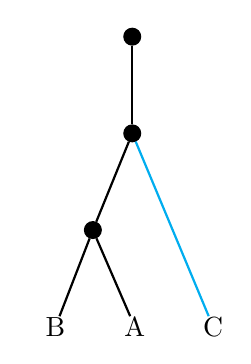
\begin{tikzpicture}[node distance={10mm}, minimum size={2mm}, inner
      sep={0pt}, thick, main/.style = {draw, circle, fill},
      color_edge/.style = {color=cyan}]
      \node[](l0){};
      \node[below = of l0](l1){};
      \node[below = of l1](l2){};
      \node[below = of l2](l3){};

      \node[main, right = 10mm of l0](root){};
      \node[main, right = 10mm of l1](abc){} edge(root);
      \node[main, right = 5mm of l2] (ba){} edge(abc);
      \node[right = 0mm of l3] (b) {B} edge(ba);
      \node[right = 10mm of l3](a) {A} edge(ba);
      \node[right = 20mm of l3] (c) {C} edge[color_edge](abc);
    \end{tikzpicture}
  \caption{Example of a rooted phylogenetic tree on the taxa $X = \{A, B, C\}$.
  The leaves are labeled with the taxa, the internal nodes don't have labels.
  Each edge can be seen as a split $S=A|B$, e.g. the cyan edge is the split $S =
  \{A, B\} | \{C\}$.}
  \label{fig:exampleTree}
\end{figure}

Phylogenetic trees are widely used to communicate evolutionary relationships
between species
\cite{mandalComparativeGenomeAnalysis2022,winkworthComparativeAnalysesComplete2022,ayala-usmaWholeGenomeDuplication2021}.
Phylogenetic trees are a type of \textit{phylogenetic networks}, of which
different types exist \cite{husonApplicationPhylogeneticNetworks2006}. Depending
on the use case, one might choose a different kind of phylogenetic network to
communicate evolutionary relationships, e.g. \textit{splits networks} or
\textit{hybridization networks}. This is especially useful when one needs to
include evolutionary events such as horizontal gene transfer or hybridization,
which are not supported by phylogenetic trees as displaying those implies
displaying loops. 

The Neighbor-Net algorithm \cite{bryantNeighborNetAgglomerativeMethod2004} is
one algorithm to construct a phylogenetic network. In the most recent version,
it works by finding a circular ordering of the taxa $X$ based on a distance matrix
$D$, calculating all splits $\Sigma$ that are compatible to that ordering and
estimating their weights \cite{bryantNeighborNetImprovedAlgorithms2023}. 

$\Sigma$ as calculated by Neighbor-Net contains $\mathcal{O}(n^2)$ splits
\cite{bryantNeighborNetImprovedAlgorithms2023}. Those splits could already be
displayed as a valid phylogenetic network, however this introduces
$\mathcal{O}(n^4)$ edges and internal nodes
\cite{bagciMicrobialPhylogeneticContext2021} that are hard to interpret.
Phylogenetic outlines provide a simplification of that by replacing internal
edges and internal nodes with a single polygon that only keeps the outermost
edges and outermost internal nodes \cite{bagciMicrobialPhylogeneticContext2021}.
In such a network, each split is either visualised by a single edge or by a pair
of parallel edges. An example of such a phylogenetic outline can be seen in
Figure~\ref{fig:outlineExample}. 

\begin{figure}
  \centering
  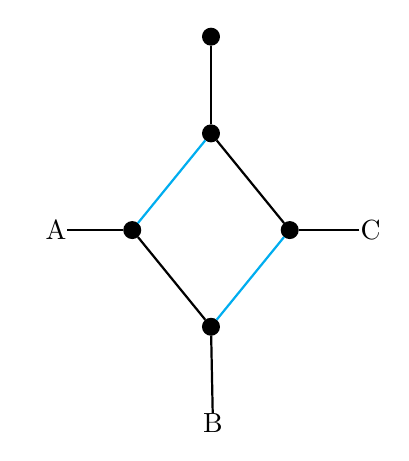
\begin{tikzpicture}[node distance={10mm}, minimum size={2mm}, inner
    sep={0pt}, thick, main/.style = {draw, circle, fill},
    color_edge/.style = {color=cyan}]
    \node[](l0){};
    \node[below = of l0](l1){};
    \node[below = of l1](l2){};
    \node[below = of l2](l3){};
    \node[below = of l3](l4){};

    \node[main, right = 20mm of l0](root){};
    \node[main, right = 20mm of l1](i1){} edge(root);
    \node[main, right = 10mm of l2](i2){} edge[color_edge](i1);
    \node[main, right = 30mm of l2](i4){} edge(i1);
    \node[main, right = 20mm of l3](i3){} edge(i2) edge[color_edge](i4);

    \node[right = 0mm of l2](a) {A} edge(i2);
    \node[right = 20mm of l4](b) {B} edge(i3);
    \node[right = 40mm of l2](c) {C} edge(i4);
  \end{tikzpicture}
  \caption{Example of a rooted phylogenetic outline on the taxa $X = \{A, B,
  C\}$. The outer nodes are labeled with the taxa, the internal nodes don't have
  labels. In this example, each edge and each pair of parallel edges can be seen
  as a split, e.g. the cyan edges depict the split $S = \{A, B\} | \{C\}$}
  \label{fig:outlineExample}
\end{figure}

\section{Phylogenetic research on \textit{Phytophthora}} 

The first scientific publication on \textit{Phytophthora} was in 1876 by
\Citeauthor{debaryResearchesNaturePotatofungus1876}
\cite{debaryResearchesNaturePotatofungus1876,kroonGenusPhytophthoraAnno2012}.
Since then, extensive research has been conducted on a variety of aspects about
this genus. Initially, as indicated by the title of the publication by
\Citeauthor{debaryResearchesNaturePotatofungus1876}, members of
\textit{Phytophthora} were thought to be fungi, but the genus is now classified
in the Phylum Pseudofungi within the kingdom Chromista
\cite{hardhamPhytophthoraCinnamomi2018,beakesEvolutionaryPhylogenyOomycete2012}.

There are many revisions of \textit{Phytophthora} phylogeny, e.g.
\cite{kroonGenusPhytophthoraAnno2012,yangExpandedPhylogenyGenus2017,abadPhytophthoraTaxonomicPhylogenetic2023a}.
Typically, the genus is divided into multiple clades, each with a numerical
identifier. The exact number and relationsips of the clades is different from
publication to publication. As I will use those clade topologies later, I will
quickly write them in Newick format.

\Citeauthor{kroonGenusPhytophthoraAnno2012} state the following topology:\\
\texttt{((((((((1, 4), 2), 5), 3), 6), 7), 8), (9, 10))}\cite{kroonGenusPhytophthoraAnno2012}

\Citeauthor{yangExpandedPhylogenyGenus2017} state the following topology:\\
\texttt{((((((((1, 4), 2), 3), 5), 7), 6), 8), (9, 10))}\cite{yangExpandedPhylogenyGenus2017}

\Citeauthor{abadPhytophthoraTaxonomicPhylogenetic2023a} state the following topolgy:\\
\texttt{(((((((((1, 2), (12, 4)), (3, 13)), 5), 6), 7), 11), 8), (9, 10))}\cite{abadPhytophthoraTaxonomicPhylogenetic2023a}

Given the rise of modern sequencing techniques, and thus the increased abundance
of available genomic data, more and more studies are also comparing different
aspects of \textit{Phytophthora} genomes, e.g. the location and content of
transposable elements and simple sequence repeats
\cite{mandalComparativeGenomeAnalysis2022}, the evolution of mitogenome
sequences involving other Peronosporaceae genomes
\cite{winkworthComparativeAnalysesComplete2022}, the diversity of
\textit{Phytophthora} genomes found in soil and water samples
\cite{catalaUseGenusSpecificAmplicon2015} or the differences in species
communities associated with soy beans
\cite{navarroComparisonSpeciesCommunities2021}.

The findings include that some \textit{Phytophthora} species are
hybrids, e.g. \textit{Phytophthora $\times$cambivora}
\cite{jungSixNewPhytophthora2017,vanpouckeUnravellingHybridizationPhytophthora2021}.
Given this information, the use of phylogenetic networks over phylogenetic trees
is becoming interesting. 

Also of interest is the concept of the two-speed genome model. Under this
hypothesis, some \textit{Phytophthora} genomes have different evolutionary
rates, i.e. the regions containing the household genes evolve slower than those
regions containing the effector genes \cite{dongTwospeedGenomesFilamentous2015}.
The fast evolving regions are gene sparse and repeat rich, the latter seems to
enable faster evolution on a molecular level with repeat induced point mutations
\cite{dongTwospeedGenomesFilamentous2015}. There is evidence for this model for
various \textit{Phytophthora} species including \textit{Phytophthora cinnamomi}
\cite{engelbrechtGenomeDestructiveOomycete2021} and \textit{Phytophthora
infestans} \cite{ayala-usmaWholeGenomeDuplication2021,dongTwospeedGenomesFilamentous2015},
but there is also evidence that not all \textit{Phytophthora} species have this
genome architecture, e.g. \textit{Phytophthora betacei}
\cite{ayala-usmaWholeGenomeDuplication2021}.

\textit{Phytophthora cinnamomi} and \textit{Phytophthora infestans} receive lots
of attention because of their impact on wildlife and agriculture:
\textit{Phytophthora cinnamomi} is reported to target over 5000 different hosts
such as avocado trees in Europe and natural vegeation in Australia
\cite{hardhamPhytophthoraCinnamomi2018,solis-garciaPhytophthoraRootRot2020},
\textit{Phytophthora infestans} is most famously known for its devestating
impact on potatoes and tomatoes \cite{ayala-usmaWholeGenomeDuplication2021}.


\section{Mash}
The phylogenies discussed above are expensive both in terms of labor and in
terms of computation: typical approaches include the prediction of conserved
genes, the alignement of the corresponding sequences and then the inference of a
phylogenetic tree, for example using bayesian inference
\cite{abadPhytophthoraTaxonomicPhylogenetic2023a,winkworthComparativeAnalysesComplete2022}.

In contrast to them, the methods used in this thesis, namely Neighbor-Joining
and the Neighbor-Net algorithm for tree and network construction, respectively,
rely on distance matrices for the involved taxa
\cite{saitouNeighborjoiningMethodNew1987,bryantNeighborNetImprovedAlgorithms2023,bryantNeighborNetAgglomerativeMethod2004}.
One could obtain such a distance matrix, e.g. by utilizing the average
nucleotide identiy (ANI) \cite{leeOrthoANIImprovedAlgorithm2016}. However, this
in turn introduces computational cost and is not suited for distantly related
species.

Another method, Mash, estimates the evolutionary distance by utilizing a concept
from web search engines from the early days of the internet: MinHash
\cite{broderResemblanceContainmentDocuments1998a,ondovMashFastGenome2016}. While
this method is about estimating the similarity between two different documents
on the world wide web, \Citeauthor{ondovMashFastGenome2016} applied the concept
to nucleotide sequences.

Let $A = a_1 a_2 \dots a_l$ be a string with length $l$ on the DNA alphabet with
$a_i = \{A, T, G, C\}$. $A$ can be decomposed into a set containing all
substrings of length $k$, so called $k$-mers, using $k(A) = \{a_i \dots
a_{i+k-1} | 1 \leq i < l-k-1\}$. Using a \textit{hash function} $h: \Omega
\rightarrow [0, H]$ with typically $H=2^{64}$ or $H=2^{128}$ on modern
computers, one can obtain the \textit{hash value} $h(i)$ for each such $k$-mer.

For the sequence $A$ the \textit{Mash sketch} $S(A)$ is the set of the
$s_{mash}$ smallest $h(i) ~ \forall i \in k(A)$. Note that the parameter
$s_{mash}$ is called $s$ in the original Mash publication
\cite{ondovMashFastGenome2016}, but as this parameter is also used in
FracMinHash with different semantics, I denote it as $s_{mash}$. One can use the
sketches of two genomes $A$ and $B$ to estimate the Jaccard similarity with 

\begin{align}
  J(A, B) = \frac{|A \cap B|}{|A \cup B|} \approx \frac{|S(A \cup B) \cap S(A) \cap S(B)|}{|S(A) \cup S(B)|}
\end{align}

This similarity can then be used to obtain a measure of distance using

\begin{align}
  D_{Mash}(A,B) = -\frac{1}{k}\ln{\frac{2J(A,B)}{1+J(A,B)}}
\end{align}

This method is widely used in different circumstances. In the original
publication, the authors created Mash sketches for all RefSeq genomes, estimated
the distances based on those and calcualted an evolutionary tree
\cite{ondovMashFastGenome2016}. Mash is also incorportated into FastANI to
estimate ANI scores, well, fast \cite{jainHighThroughputANI2018}.

A third use case for Mash is the creation of phylogenetic contexts using
phylogenetic outlines \cite{bagciMicrobialPhylogeneticContext2021} in
metagenomic studies. Here, one sequences all DNA found in a given sample, e.g.
soil or sea water, and assembles (draft) genomes from the acquired reads
\cite{kuninBioinformaticianGuideMetagenomics2008}. Outlines help with
identifying the species to which the draft genome belongs. For this, the
phylogenetic context is established by placing the draft genome in a
phylogenetic outline using all sequences from a reference databases that have a
Mash distance to the query below a user defined threshold
\cite{bagciMicrobialPhylogeneticContext2021}.

Mash itself is implemented in a tool called \texttt{mash}
\cite{ondovMashFastGenome2016}. For convenience, there exists also a tool called
\texttt{mashtree} \cite{katzMashtreeRapidComparison2019} which utilizes Mash to
directly calculate distances and a phylogenetic tree given some input sequences.

\section{FracMinHash}
Mash is not the only method in the area of \textit{locality sensitive hashing}.
A recently published method is called FracMinHash by
\Citeauthor{irberLightweightCompositionalAnalysis2022}
\cite{irberLightweightCompositionalAnalysis2022} and aims to tackle some of the
issues with Mash, namely the fact that Mash is not optimal for containment
estimation and that it is not optimal for distance estimation for genomes with
different sizes
\cite{heraDerivingConfidenceIntervals2023,koslickiImprovingMinHashContainment2019}.

The key idea of FracMinHash is to define a threshold $\frac{H}{s}$ with $H$
being the largest value that $h$ can produce and $s$ a user defined scaling
parameter with $0 < s \leq H$ such that a FracMinHash sketch only contains hash
values below that threshold. As shown in Section~\ref{sec:res}, the sketch size can be
approximated by $\frac{n}{s}$ where $n$ is the size of the input sequence
\cite{irberLightweightCompositionalAnalysis2022,heraDerivingConfidenceIntervals2023}.


Formally, the FracMinHash sketch is defined as 

\begin{align}
  \mathbf{FRAC}_s(A) = \{h(i) \leq \frac{H}{s} | \forall i \in k(A)\}
\end{align}

This approach has the advantage that the sketching can be applied to streams: it
is known if a hash is part of the sketch as soon as the $k$-mer is hashed. This
also applies when calculating the intersection between two sketches. 

In Mash, to estimate the Jaccard index, it is required to also find the
$s_{mash}$ smallest overall hashes of the two input sequences, i.e. $S(A \cup
B)$. This is not needed for FracMinHash, as all hashes that are part of the
input sketches already satisfy the condition $\leq \frac{H}{s}$. Thus, the
Jaccard estimation (including a factor correcting for bias) is given in
\cite{heraDerivingConfidenceIntervals2023} as

\begin{align}
  J_{frac} = \frac{\hat{J}_{frac}}{1 - (1 - s)^{|A \cup B|}}
\end{align}

with

\begin{align}
  \hat{J}_{frac}(A, B) = \frac{|\mathbf{FRAC}_s(A) \cap \mathbf{FRAC}_s(B)|}{|\mathbf{FRAC}_s(A) \cup \mathbf{FRAC}_s(B)|}  
\end{align}

This Jaccard index can be used to calculate evolutionary distances, for which
the FracMinHash publications follow again an approach different to Mash. Mash
uses a Poisson model that assumes that all $k$-mers mutate independently
\cite{ondovMashFastGenome2016,heraDerivingConfidenceIntervals2023,fanAssemblyAlignmentfreeMethod2015},
whereas FracMinHash assumes a simple model in which each nucleotide $a_i$ of a
sequence $A$ mutates at a fixed rate $p$
\cite{heraDerivingConfidenceIntervals2023}. The authors note that such a
mutated sequence $A'$ has an average nucleotide identity (ANI) of $1-p$ to $A$.
As the inverse can be used to calculate a distance from any similarity ($D = 1 -
I$), I will denote $p$ in the following as $D_{frac}$. Following this, the
authors define an estimation of the distance in
\cite{heraDerivingConfidenceIntervals2023} as

\begin{align}
  D_{frac}(A, B) = 1 - (\frac{2J_{frac}(A,B)}{1+J_{frac}(A, B)})^{\frac{1}{k}}
\end{align}

FracMinHash also defines a containment index and the corresponding distance:
\begin{align}
  C_{frac}(A, B) = \frac{|\mathbf{FRAC}_S(A) \cap \mathbf{FRAC}_s(B)|}{|\mathbf{FRAC}_S(A)| (1-(1-s)^{|A|})}
\end{align}
\begin{align}
  D=1-C_{frac}^{\frac{1}{k}}
\end{align}

FracMinHash is implemented in a tool called \texttt{sourmash}
\cite{irberLightweightCompositionalAnalysis2022,irberDecentralizingIndicesGenomic2020}.
For the purpose of this thesis, I have implemented the method in
\texttt{fmhdist} to obtain phylogenetic outlines as described in
\cite{bagciMicrobialPhylogeneticContext2021}.

\cleardoublepage

%% 
% !TEX root = thesis.tex
%%%%%%%%%%%%%%%%%%%%%%%%%%%%%%%%%%%%%%%%%%%%%%%%%%%%%%%%%%%%%%%%%%%%
% Materials and Methods
%%%%%%%%%%%%%%%%%%%%%%%%%%%%%%%%%%%%%%%%%%%%%%%%%%%%%%%%%%%%%%%%%%%%

\chapter{Material and Methods}
  \label{sec:matmet}

\section{Libraries used for Implementation}
The generation of phylogenetic outlines using FracMinHash was implemented using
\texttt{java-17}, \texttt{jloda3} 1.0.0, \texttt{splitstree6} 1.0.0
\cite{husonApplicationPhylogeneticNetworks2006} and
\texttt{openapi-generator-maven-plugin} 6.3.0. For the hash functionality,
\texttt{zero-allocation-hashing} 0.16 is used. \todo{Check: Do I need a full
list or just the main contributers? Do I need a reference for each?}


\section{Benchmarking the Hash Functions}
To get an understanding of which hash function performs best in terms of
runtime, the \texttt{jmh} benchmarking framework 1.37 was used to benchmark the
following hash functions:

\begin{itemize}
  \item MurMur3 \todo{add citation/links to all hash functions}
  \item XX3
  \item XX64
  \item XX128
  \item City 1.1
  \item Farm 1.0
  \item Farm 1.1
  \item Wy 3
  \item Metro
\end{itemize}
 
While other hash function implementations were considered, the implementation of
all hash functions is given by \texttt{zero-allocation-hashing} 0.16. The
benchmark was executed in throughput mode using a fork count of 2. Besides that,
default parameters were used.


\section{Datasets used}
To evaluate properties of FracMinHash, analysis was performed using different
data sets. 

The first dataset (\textbf{A}) consists of 128 different \textit{Phytophthora}
genomes. The list is taken from \cite{mandalComparativeGenomeAnalysis2022}
without further modifications. Genomes were downloaded from NCBI uding the
\texttt{datasets} utility \cite{sayersDatabaseResourcesNational2022} using the
accession codes listed in that study.

The second dataset (\textbf{B}) consists of 72 mtDNA sequences of
\textit{Phytophthora}
and other Oomycetes of the Peronosporaceae family. The list is taken without
further modifications from Supplementary Table 1 from
\cite{winkworthComparativeAnalysesComplete2022}. Genomes were downloaded from
NCBI using the Entrez interface \cite{sayersDatabaseResourcesNational2022} using
the accession codes listed in that study, appended by the identifier of the most
recent version for that accession code.

The third dataset (\textbf{C}) consists of all 64 \textit{Phytophthora}
reference sequences in the NCBI databasase ("reference") as well as five
different query sequences that are typically found in soil samples of avocado
orchards that are infected with \textit{Phytophthora cinnamomi}
\cite{solis-garciaPhytophthoraRootRot2020}. Those query sequences are divided
into two bacterial genomes, two fungal and one \textit{Phytophthora cinnamomi}
genome:

\begin{itemize}
  \item fungal: \textit{Mortierella claussenii} - GCA\_022750515.1
  \item bacterial: \textit{Thermogemmatispora aurantia} - GCA\_008974285.1
  \item fungal: \textit{Venturia carpophila} - GCA\_014858625.1
  \item bacterial: \textit{Pseudomonas syringae} - GCA\_018394375.1
  \item fungal: \textit{Phytophthora cinnamomi} - GCA\_001314365.1
\end{itemize}

The full list of reference sequences can be found in the appendix \todo{ref}.
The reference sequences were downloaded using the web interface (Filter:
reference sequences), the query sequences were downloaded using the
\texttt{datasets} utility.



\section{Comparison with published Phylogenies}
\cite{mandalComparativeGenomeAnalysis2022} displays a rooted phylogenetic tree
in Figure 4 that was generated using the \texttt{mashtree}
\cite{katzMashtreeRapidComparison2019,ondovMashFastGenome2016}. Unfortunately,
the corresponding distance matrix or a serialized version of the tree are not
available. Thus, the data needs to be re-computed. For this, the
\texttt{mashtree\_bootstrap.pl} 1.4.6 was applied to dataset A as described by
\cite{mandalComparativeGenomeAnalysis2022}, additionally the distance matrix was
saved using the \texttt{--outmatrix} parameter.

Distance matrices for dataset A using the FracMinHash method were calculated using different
combinations of the scaling parameter $s$ and $k$-mer size $k$:

\begin{itemize}
  \item $k=19$, $s=2000$
  \item $k=20$, $s=2000$
  \item $k=21$, $s=2000$
  \item $k=25$, $s=2000$
  \item $k=30$, $s=2000$
  \item $k=21$, $s=500$
  \item $k=21$, $s=1000$
  \item $k=21$, $s=40000$
\end{itemize}

To ensure comparability with the \texttt{mashtree} results, the same hashing
function (MurMur) and random seed (42) were used to calculate the sketches
\cite{katzMashtreeRapidComparison2019,ondovMashFastGenome2016}.

For all distance matrices, SplitsTree 6.0.0-alpha
\cite{husonApplicationPhylogeneticNetworks2006} was used to obtain trees, splits
and outlines. Trees were calculated using the Neighbor Joining method
\cite{saitouNeighborjoiningMethodNew1987}. Splits were obtained using the
Neighbor Net method
\cite{bryantNeighborNetAgglomerativeMethod2004,bryantNeighborNetImprovedAlgorithms2023}
using the default parameters. Based on this, a phylogenetic outline was
calculated \cite{bagciMicrobialPhylogeneticContext2021}.



\section{Split difference analysis}
\label{sec:splitanalysis}
To analyse the differences between the phylogenetic outline based on the Mash
distances and the outlines based on FracMinHash further, the splits were
analysed in details. For this, the splits were exported from SplitsTree
6.0.0-alpha \cite{husonApplicationPhylogeneticNetworks2006} using the plain text
format.

Those files were processed with the script \texttt{compare\_splity.py}. This is
based on \texttt{python} 3.12 and \texttt{pandas} 2.1.4
\cite{PandasdevPandasPandas2024,mckinneyDataStructuresStatistical2010}. All sets
of splits are compared pairwise, that is for two sets $\Sigma_A$ and $\Sigma_B$,
the following properties are calculated:

\begin{itemize}
  \item the total sum of weight for all splits in $\Sigma_A$ and $\Sigma_B$,
  respectively: $\sum_{s \in \Sigma_A}{\omega(s)}$ and $\sum_{s \in
  \Sigma_B}{\omega(s)}$ 
  \item the number of splits in $\Sigma_A / \Sigma_B$ and the number of splits
  in $\Sigma_B / \Sigma_A$
  \item the total weight difference associated with the remaining splits, i.e.
  $\sum_{s \in \Sigma_A / \Sigma_B}{\omega(s)}$ and $\sum_{s \in \Sigma_B /
  \Sigma_A}{\omega(s)}$
  \item the Robinson-Foulds distance
  \cite{robinsonComparisonPhylogeneticTrees1981} of the two sets of splits, i.e.
  $D_{RF} = \frac{1}{2}|(\Sigma_A / \Sigma_B) \cup (\Sigma_B / \Sigma_A)|$
\end{itemize}

The script outputs a list of the diverging splits sorted by the weight of the
split. Each split is formatted as a list of taxa names on the smaller side of
the split sorted alphabetically and joined using the "|" symbol such that the
split can be searched in SplitsTree 6 using the regular expression search.



\section{Reproducing phylogenies for shorter sequences}
To get an idea of the practical lower boundarys of FracMinHash in terms of input
genome size, dataset B was sketched. As this dataset consists of just a single
long FASTA file, it was split into its records using \texttt{split-fasta} 1.0.0
\todo{check citation}. The files were then sketched with FracMinHash using
$k=21$, $s \in \{1, 10, 50, 100, 1000\}$ and the \todo{redo with most recent
implementation, check sketch sizes. Redo because I don't know with which version
the sketches were computed, thus I don't know how to calculate the sizes.}
MurMur hash function with random seed 42.

Given the calculated distances, SplitsTree 6.0.0-alpha
\cite{husonApplicationPhylogeneticNetworks2006} was used to obtain trees, splits
and outlines. Trees were calculated using the Neighbor Joining method
\cite{saitouNeighborjoiningMethodNew1987}. Splits were obtained using the
Neighbor Net method
\cite{bryantNeighborNetAgglomerativeMethod2004,bryantNeighborNetImprovedAlgorithms2023}
using the default parameters. Based on this, a phylogenetic outline was
calculated \cite{bagciMicrobialPhylogeneticContext2021}.


\section{Calculating distances of distantly related genomes and genomes with different sizes}
To analyse the claim that FracMinHash works better for genomes of different
sizes \todo{ensure this claim is cited at least once!}, both reference and query
sequences of dataset C were sketched, distances calculated and the results
compared. 

\subsection*{Sketching using FracMinHash}
\label{sec:intersectionlog}
Reference and query sequences were sketched with $k=21$, $s=2000$ using FarmHash
with random seeds $rs \in \{10, 20, 30, 40, 50\}$. As the default sketch size
for Mash is 10000 \cite{ondovMashFastGenome2016} and to ensure that it is not
the fact that the relevant sketches are just larger, additional sketching with
$s=500$ (which aims to bring the sketch size of the bacterial query sequences to
10000) and $s=3500$ (which aims to bring the sketch size of the fungal query
sequences to 10000) was performed. Using the sketches, the distance matrix was
calculated. For this, the implementation was changed such that an additional log
is created that lists all empty intersections when calculating the intersection
of the two sketches.

\subsection*{Sketching using MashTree}
To obtain a base value to compare agains, \texttt{mashtree} 1.4.6
\cite{katzMashtreeRapidComparison2019,ondovMashFastGenome2016} was applied with
hash seed $rs \in \{10, 20, 30, 40, 50\}$, \texttt{--outmatrix} and the
\texttt{--save-sketches} parameter. The resulting sketches were then also
converted into JSON format using \texttt{mash info -d}.

\subsection*{Visual comparison and split differences}
Given all calculated distances, SplitsTree 6.0.0-alpha
\cite{husonApplicationPhylogeneticNetworks2006} was used to obtain trees, splits
and outlines. Trees were calculated using the Neighbor Joining method
\cite{saitouNeighborjoiningMethodNew1987}. Splits were obtained using the
Neighbor Net method
\cite{bryantNeighborNetAgglomerativeMethod2004,bryantNeighborNetImprovedAlgorithms2023}
using the default parameters. Based on this, a phylogenetic outline was
calculated \cite{bagciMicrobialPhylogeneticContext2021}.

The splits were then also analysed using the script outlined in Section
\ref{sec:splitanalysis}.

\subsection*{Obtaining reference values}
As there are no published phylogenies for dataset C that enable a comparison, I
need a different ground truth to compare the results of above distance
calculation against. As the aim for this experiment is to analyze the influcence
of different genome sizes of distantly related organisms, I have limited this
analysis to the five query sequences of dataset C and the reference genome for
\textit{Phytophthora infestans} (GCF\_000142945.1) as this is one of the largest
genomes in the set of reference sequences. For those sequences, I have prepared
two different values to compare against.

The first ist the Average Nucleotide Identity (ANI)
\cite{konstantinidisGenomeBasedTaxonomyProkaryotes2005} calculated with
\texttt{OrthoANI} \cite{leeOrthoANIImprovedAlgorithm2016} using the default
parameters with \texttt{BLAST+} 2.14.1
\cite{camachoBLASTArchitectureApplications2009} as the aligner.

The second is the Average Amino Acid Identity (AAI) calculated with the
\texttt{Enveomics Collection} online resource
\cite{rodriguez-rEnveomicsCollectionToolbox2016} using default parameters. As
this requires amino acid sequences as input and those are not available for the
\textit{Venturia carpophila} and \textit{Phytophthora cinnamomi} sequences, they
were predicted using the \texttt{gmes\_petap.pl} script provided in the
\texttt{GeneMark ES} 4.72 package \cite{lomsadzeGeneIdentificationNovel2005}
using the default parameters and extracted using the \texttt{gffread} utility
0.12.7 \cite{perteaGFFUtilitiesGffRead2020}.


\subsection*{Calculating empty intersections}
When the sketch intersections are empty, the estiamted Jaccard similarity is
always 0. Mash does not only calculate the sketch intersections, but also
intersects that result with the sketch of the union of the two input sketches
\cite{ondovMashFastGenome2016}. This increases the chances of getting a Jaccard
estimation of 0. 

To test this, I have prepared a the script \texttt{get\_empty\_intersections.py}
which takes a list of Mash sketches in JSON format and outputs all pairs for
which the numerator of the Jaccard estimation is empty.

The same is possible using the added log output generated by the distance
calculation described in Section \ref{sec:intersectionlog}.

Using the five different random seeds, we can convert this output into a table
that lists the number of empty intersections for each pairwise calculation. 



\section{Hash Density analysis}

\cleardoublepage

%%
% !TEX root = thesis.tex
%%%%%%%%%%%%%%%%%%%%%%%%%%%%%%%%%%%%%%%%%%%%%%%%%%%%%%%%%%%%%%%%%%%%
% Results
%%%%%%%%%%%%%%%%%%%%%%%%%%%%%%%%%%%%%%%%%%%%%%%%%%%%%%%%%%%%%%%%%%%%

\chapter{Results}
  \label{sec:res}

\section{Implementation of FracMinHash}
To evaluate several aspects of FracMinHash, a Java implementation called
\texttt{fmhdist} was created in the context of this thesis. This tool has five
main functions that are described in the following.

\subsection*{\texttt{fmhdist sketch}}

\texttt{fmhdist sketch} takes a list of paths to a sequence file and calculates
the FracMinHash sketch for each sequence. The user can set the $k$-mer size $k$
(defaults to $21$), the scaling parameter $s$ (defaults to $2000$), the hash
function (defaults to \texttt{farm}) and the random seed for the hash function
(defaults to $42$). The user can also specify the output path and weither or not
they want to receive the hash coordinates for each sketch.

\subsection*{\texttt{fmhdist dist}}

\texttt{fmhdist sketch} takes a list of paths to sketch files and calculates the
distance based on the estimated Jaccard index, the distance based on the
estimated containment index
\cite{heraDerivingConfidenceIntervals2023,irberLightweightCompositionalAnalysis2022}
and the Mash distance based on the estimated Jaccard index
\cite{ondovMashFastGenome2016}. The distance matrices are stored as a Nexus file
and can be imported in tools such as SplitsTree 6 to obtain the phylogenetic
outline or tree.

\subsection*{\texttt{fmhdist db}}

\texttt{fmhdist db} takes a list of NCBI accession codes and creates a reference
dabatase in SQLite format. This database contains the sketches for each taxon
listed in the input as well as the full taxonomic tree that includes those taxa.
If multiple accession codes point to the same taxon, only the first is inserted
in the database. For the sketching, the user has the same choice of parameters
as for \texttt{fmhdist sketch}.

\subsection*{\texttt{fmhdist ref-dist}}

\texttt{fmhdist ref-dist} takes a set of query sketches, a threshold and a
reference database either as produced by \texttt{fmhdist db} or as a list of
sketches. For each query sketch, the pairwise distance based on the Jaccard
estimation is calculated. Those reference sequences that have a distance below
the threshold to any of the query sequences are included in a final pairwise
distance calculation. This works identically to the \texttt{fmhdist dist}
command.

\subsection*{\texttt{fmhdist outline}}

\texttt{fmdist outline} takes a distance matrix in Nexus format (e.g. as
produced by \texttt{fmhdist dist}) and calculates a phylogenetic outline based
on those distances. The resulting image is saved as a scalable vector graphic
(SVG) and can be further edited by the user using an SVG editor of choice.

\section{Phylogenies for dataset \textbf{A} cluster by clade} The trees and
outlines generated by \texttt{fmhdist} and \texttt{mashtree}, respectively, and
\texttt{SplitsTree} 6.3.20
\cite{husonApplicationPhylogeneticNetworks2006,bagciMicrobialPhylogeneticContext2021}
for dataset \textbf{A }generally represent the clade association and the
relationships between clades well. All included taxa are clustered with their
corresponding clade members
\cite{abadPhytophthoraTaxonomicPhylogenetic2023a,yangExpandedPhylogenyGenus2017}.

The dataset includes several taxa that are represented by multiple different
sequences. This relationship can also be read from the produced trees and
outlines.

\subsection*{Trees}
The tree that was calculated using the re-computed Mash distance for dataset
A is depicted in Figure~\ref{fig:mandalMashTree}. Clade clusters are well
defined and in line with literature
\cite{abadPhytophthoraTaxonomicPhylogenetic2023a,yangExpandedPhylogenyGenus2017}.
Using Newick notation, this tree indicates the following topology: 

\texttt{(((((1, 2), 4), 5), (((7, 3), 6), 8)), 10)}

We can see that the relationships of the inner clades 1, 2 and 4 are in line
with literature, the clades 3, 6, 7 and 8 form a monophyletic group which is not
in line with literature.
\cite{abadPhytophthoraTaxonomicPhylogenetic2023a,yangExpandedPhylogenyGenus2017}.

\begin{figure}
  \centering
  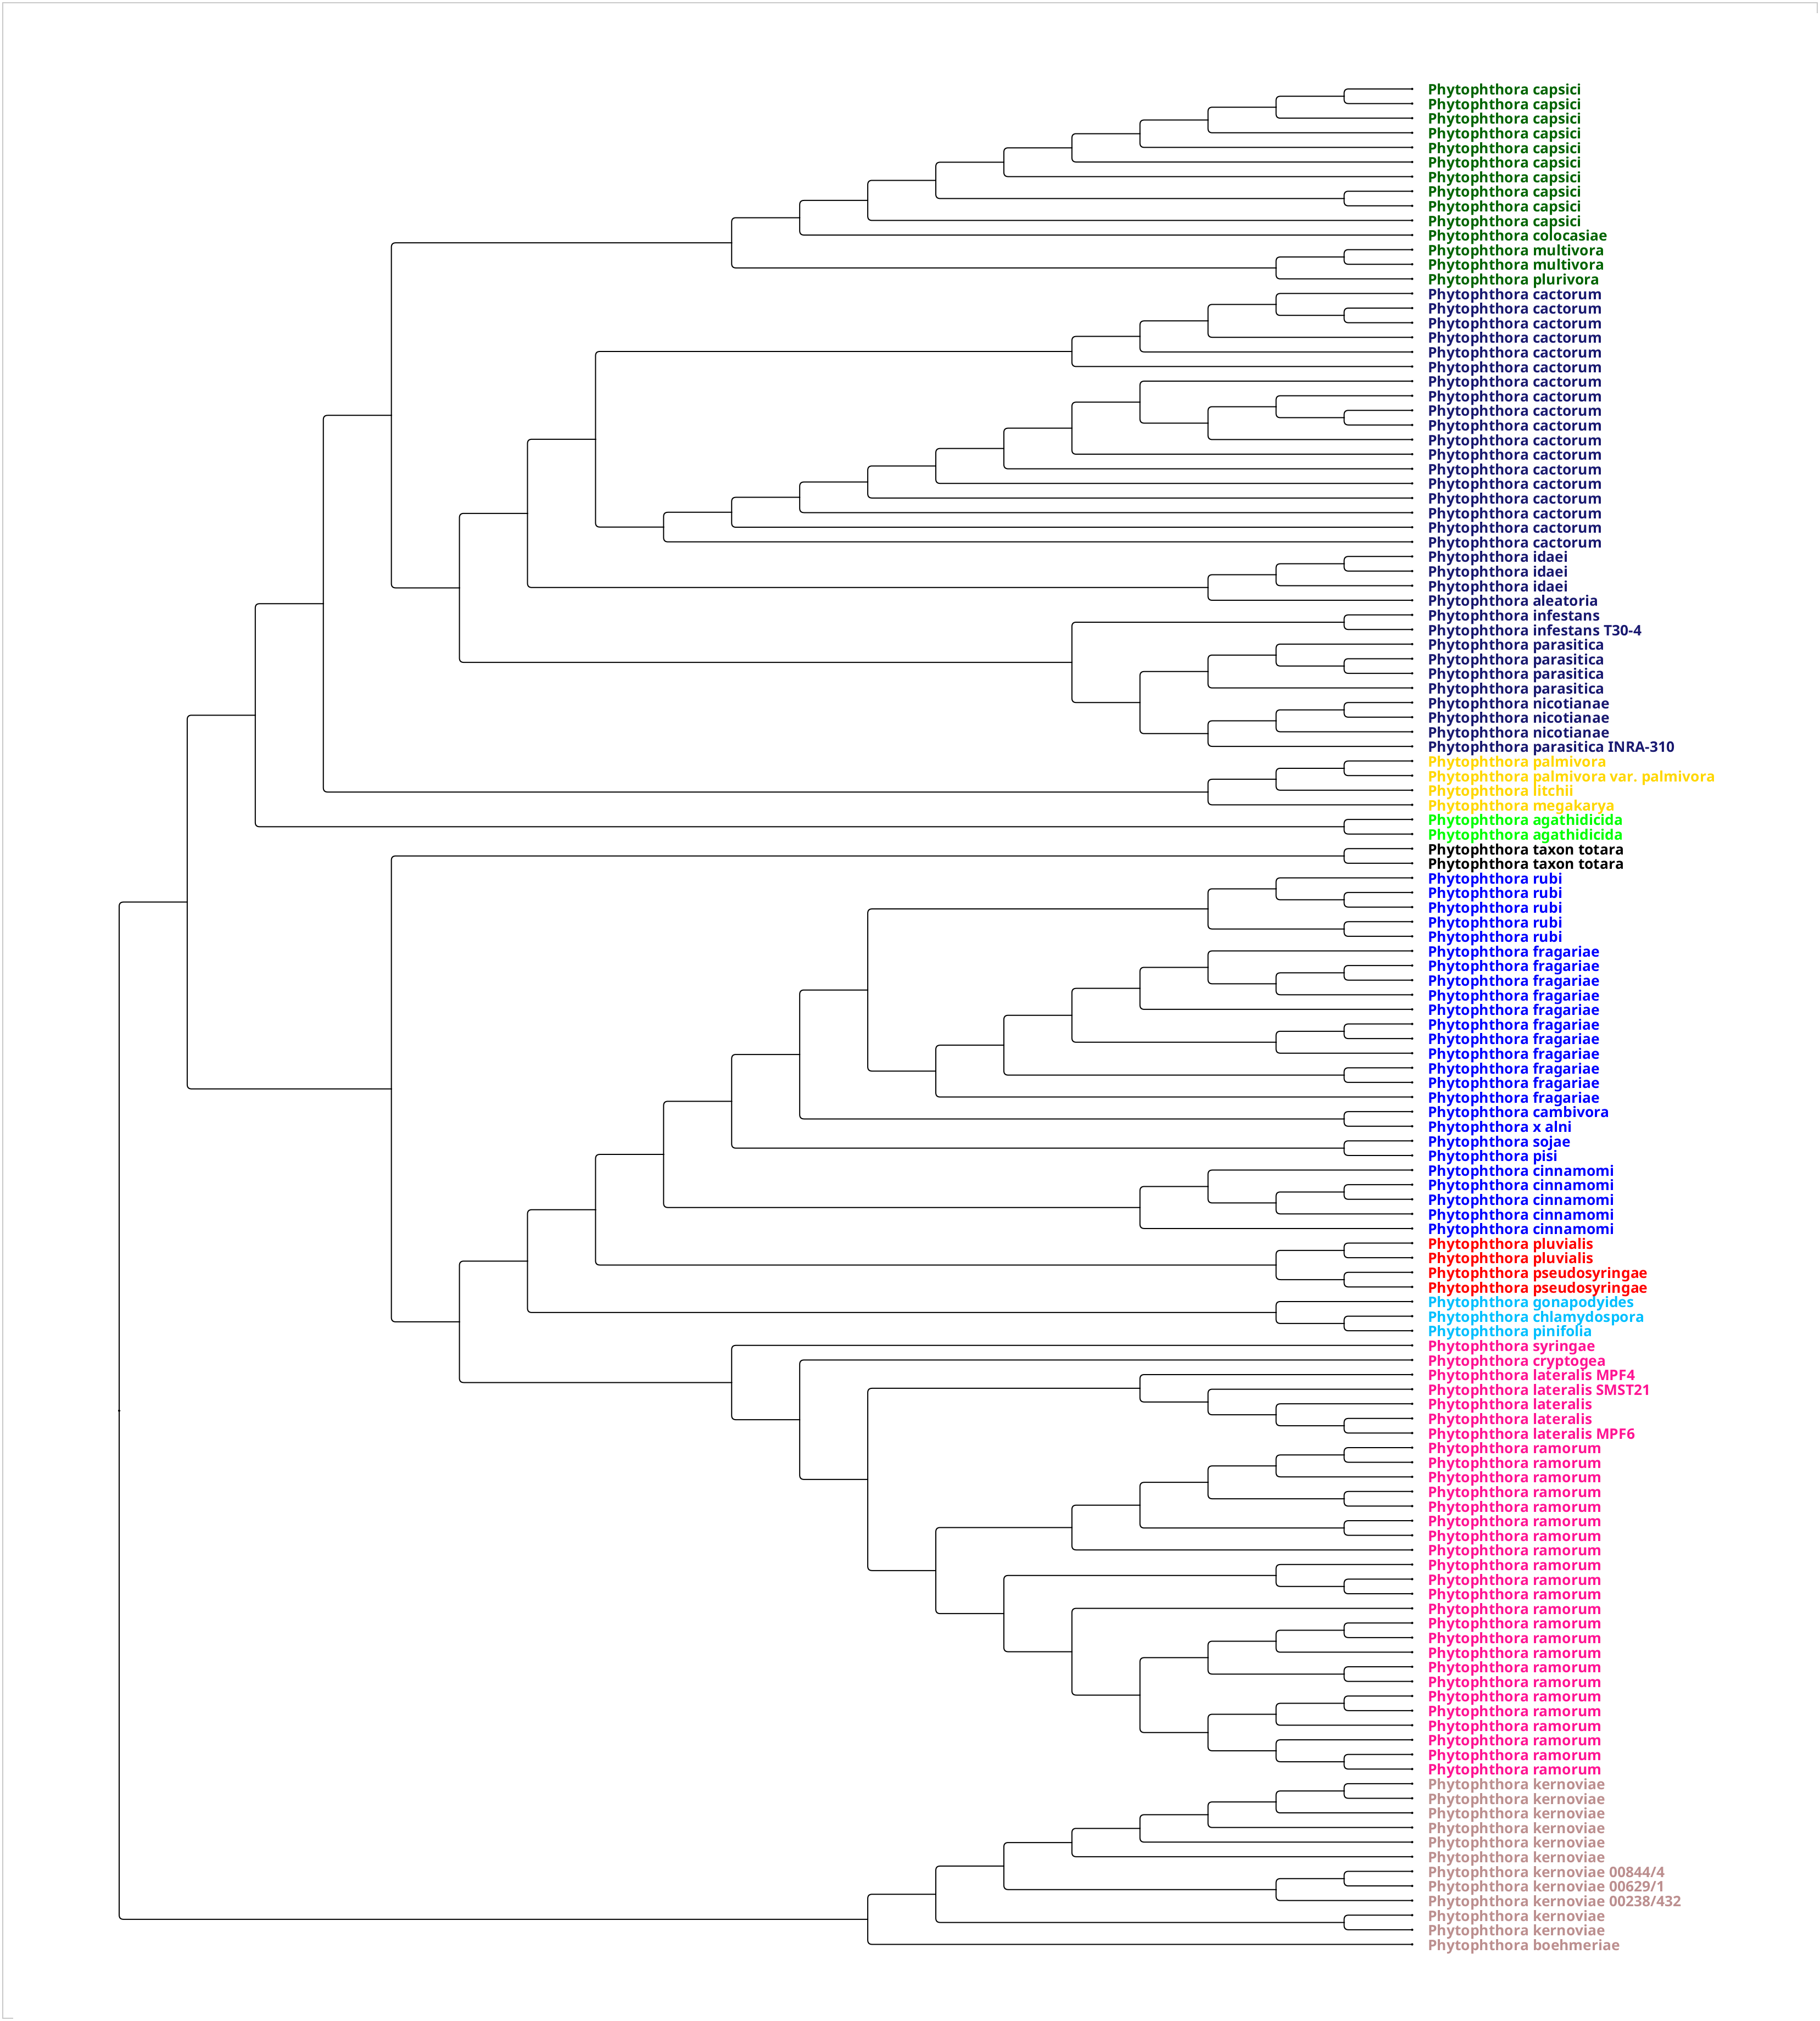
\includegraphics[width=0.9\textwidth]{figures/mashtree_mandal_tree_k21_s2000.png}
  \caption[Phylogenetic tree based on distances of dataset \textbf{A} calculated with
  \texttt{mashtree}]{Phylogenetic tree based on distances of dataset \textbf{A}
  calculated with
  \texttt{mashtree}
  \cite{ondovMashFastGenome2016,katzMashtreeRapidComparison2019}. Taxa are
  colored according to clade membership
  \cite{abadPhytophthoraTaxonomicPhylogenetic2023a}. The tree is rooted with
  clade 10 as outputgroup.}
  \label{fig:mandalMashTree}
\end{figure}

The tree that was calculated using the FracMinHash distance for dataset A is
depicted in Figure~\ref{fig:mandalFmhdistTree}. Again, clade clusters are well
defined and in line with literature.
Using Newick notation, this tree indicates the following topology:

\texttt{(((((1, 2), 4), 5), (3, ((6, 7), 8))), 10)}

Again, the relationships of the clades 1, 2 and 4 are in line with literature
\cite{abadPhytophthoraTaxonomicPhylogenetic2023a,yangExpandedPhylogenyGenus2017}.
the clades 3, 6, 7 and 8 form a monophyletic group which is not in line with
literature.

\begin{figure}
  \centering
  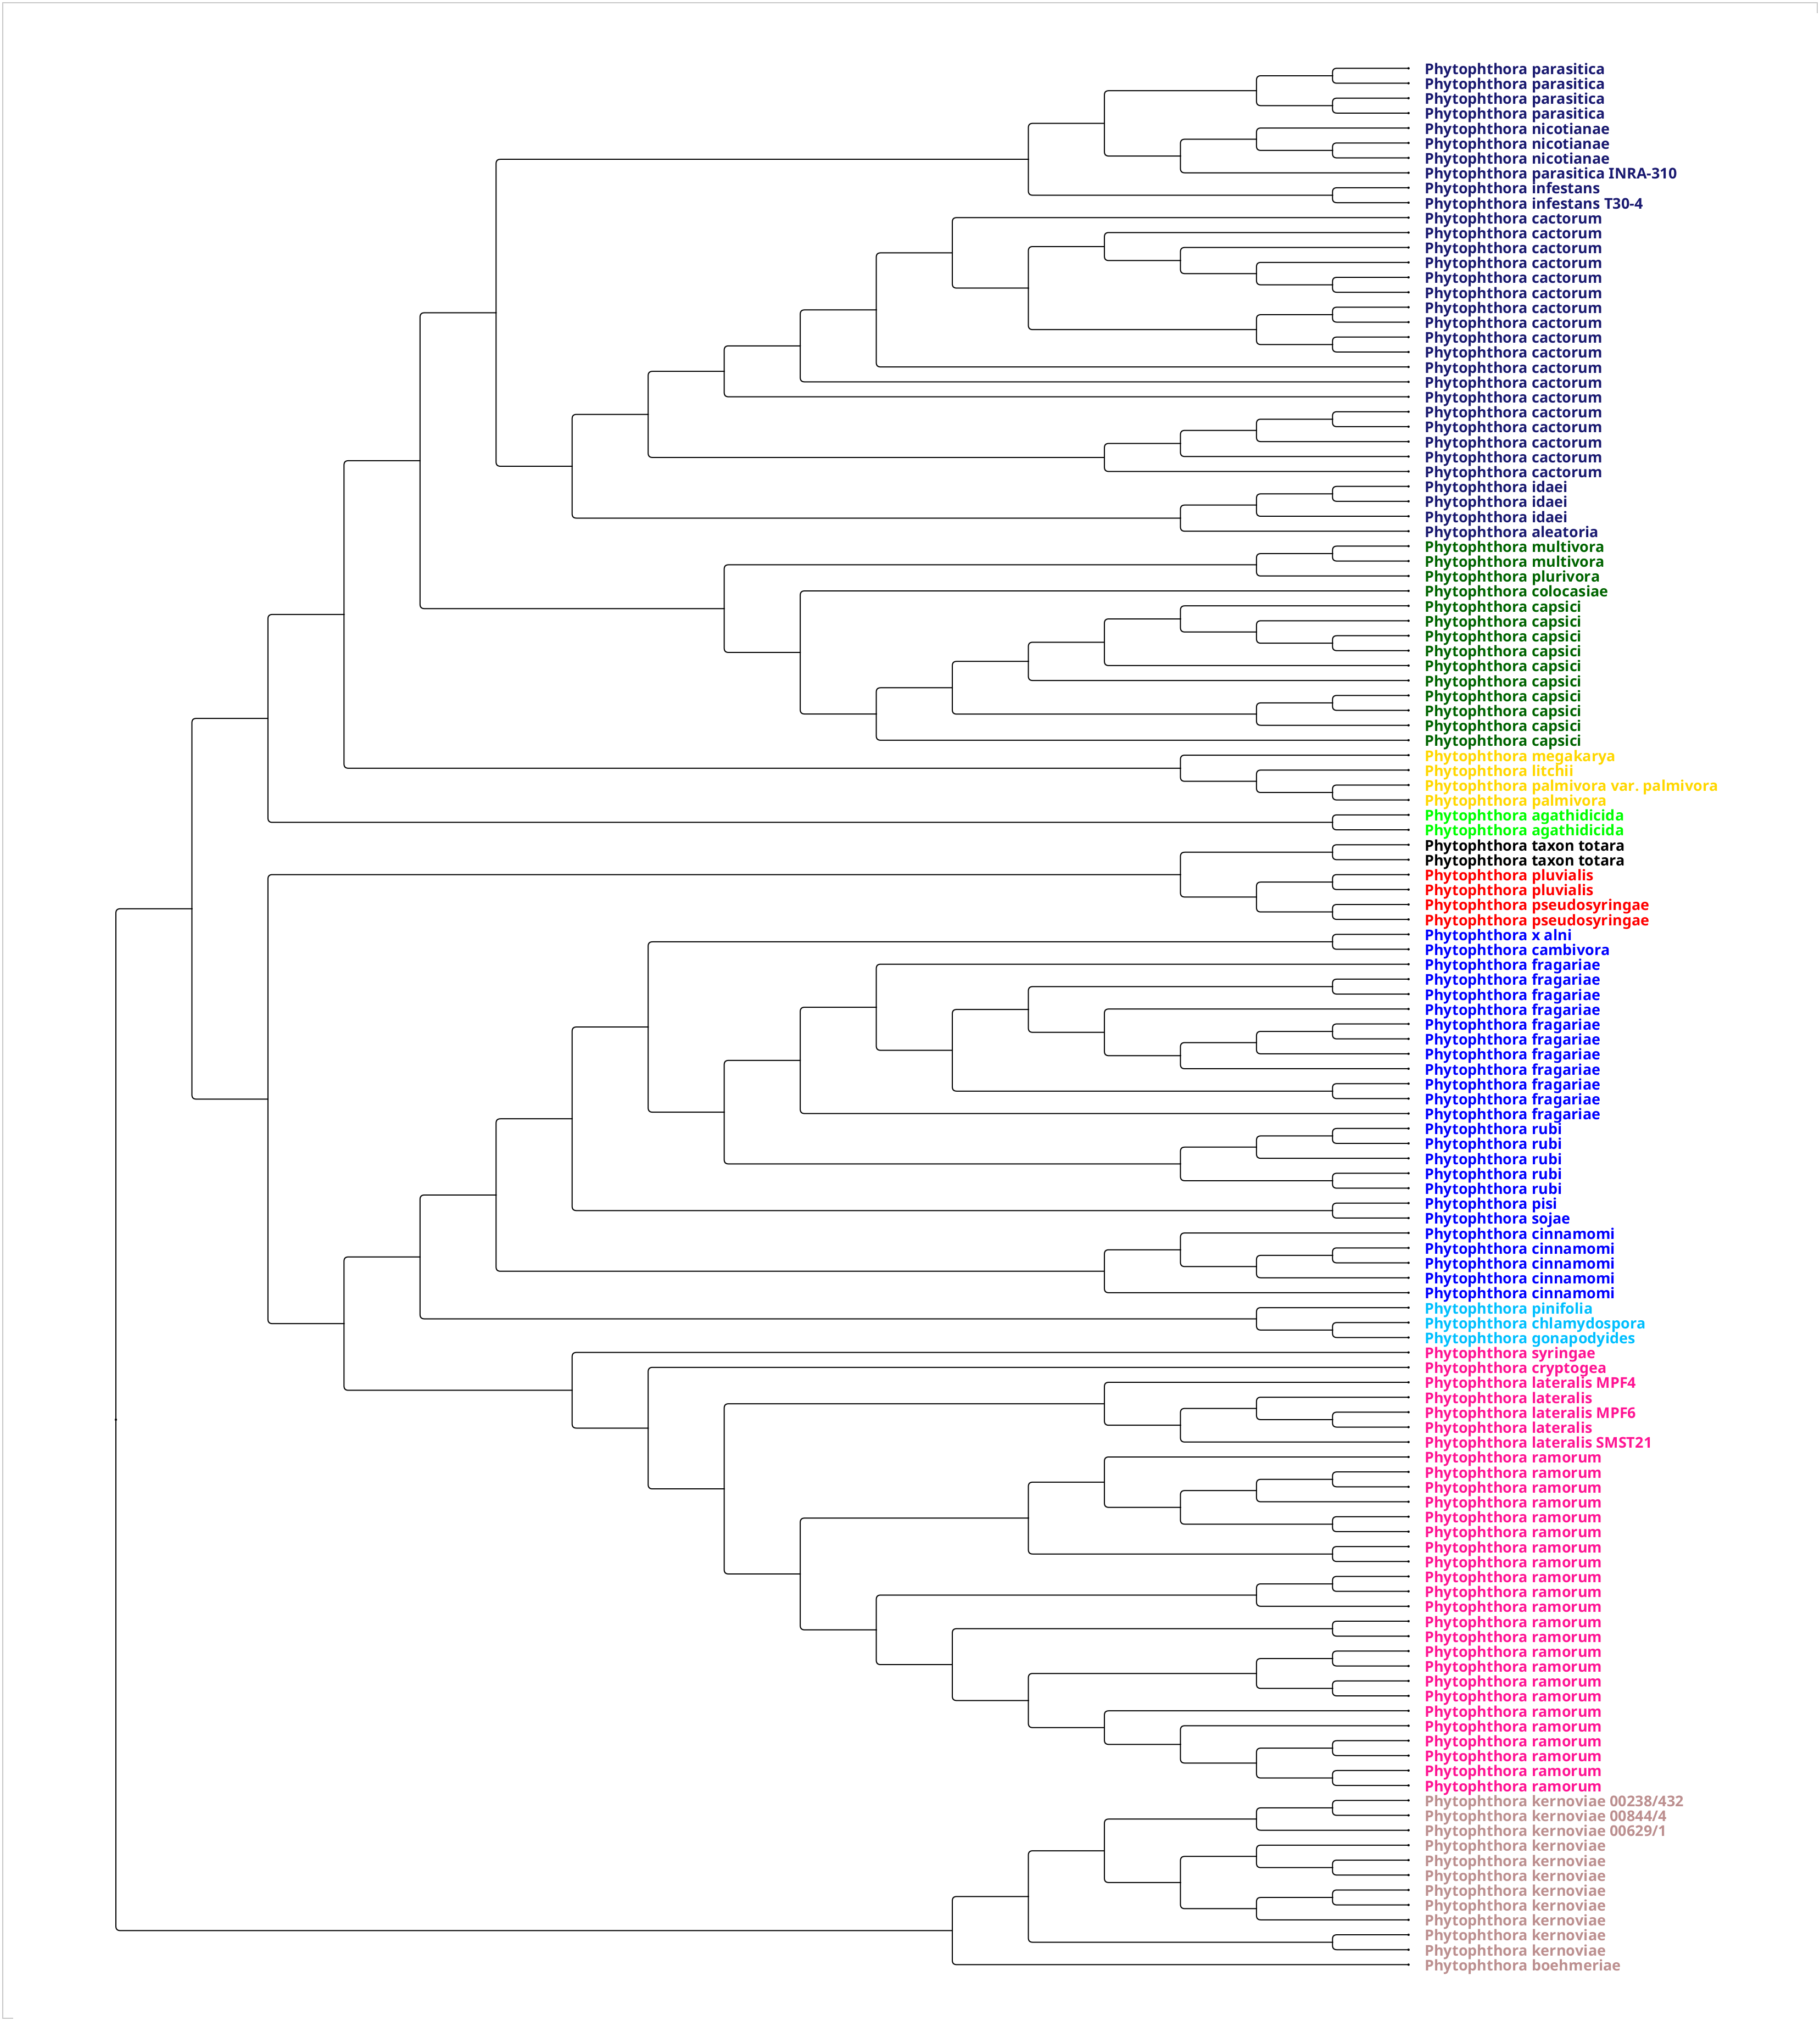
\includegraphics[width=0.9\textwidth]{figures/fmhdist_mandal_tree_k21_s2000.png}
  \caption[Phylogenetic tree based on distances of dataset \textbf{A} calculated
  with \texttt{fmhdist}]{Phylogenetic tree based on distances of dataset
  \textbf{A} calculated with \texttt{fmhdist}. Taxa are colored according to
  clade membership \cite{abadPhytophthoraTaxonomicPhylogenetic2023a}. The tree
  is rooted with clade 10 as outgroup.}
  \label{fig:mandalFmhdistTree}
\end{figure}

\todo{maybe reference consensus network here?}

\subsection*{Outlines}
The phylogenetic outline that was calculated using the re-computed Mash
distances for dataset A is shown in Figure~\ref{fig:mandalMashOutline}. Similar
to the trees, clusters are well defined and in line with literature
\cite{abadPhytophthoraTaxonomicPhylogenetic2023a,yangExpandedPhylogenyGenus2017}.
The outline also visualizes the subclades well.

\begin{figure}
  \centering
  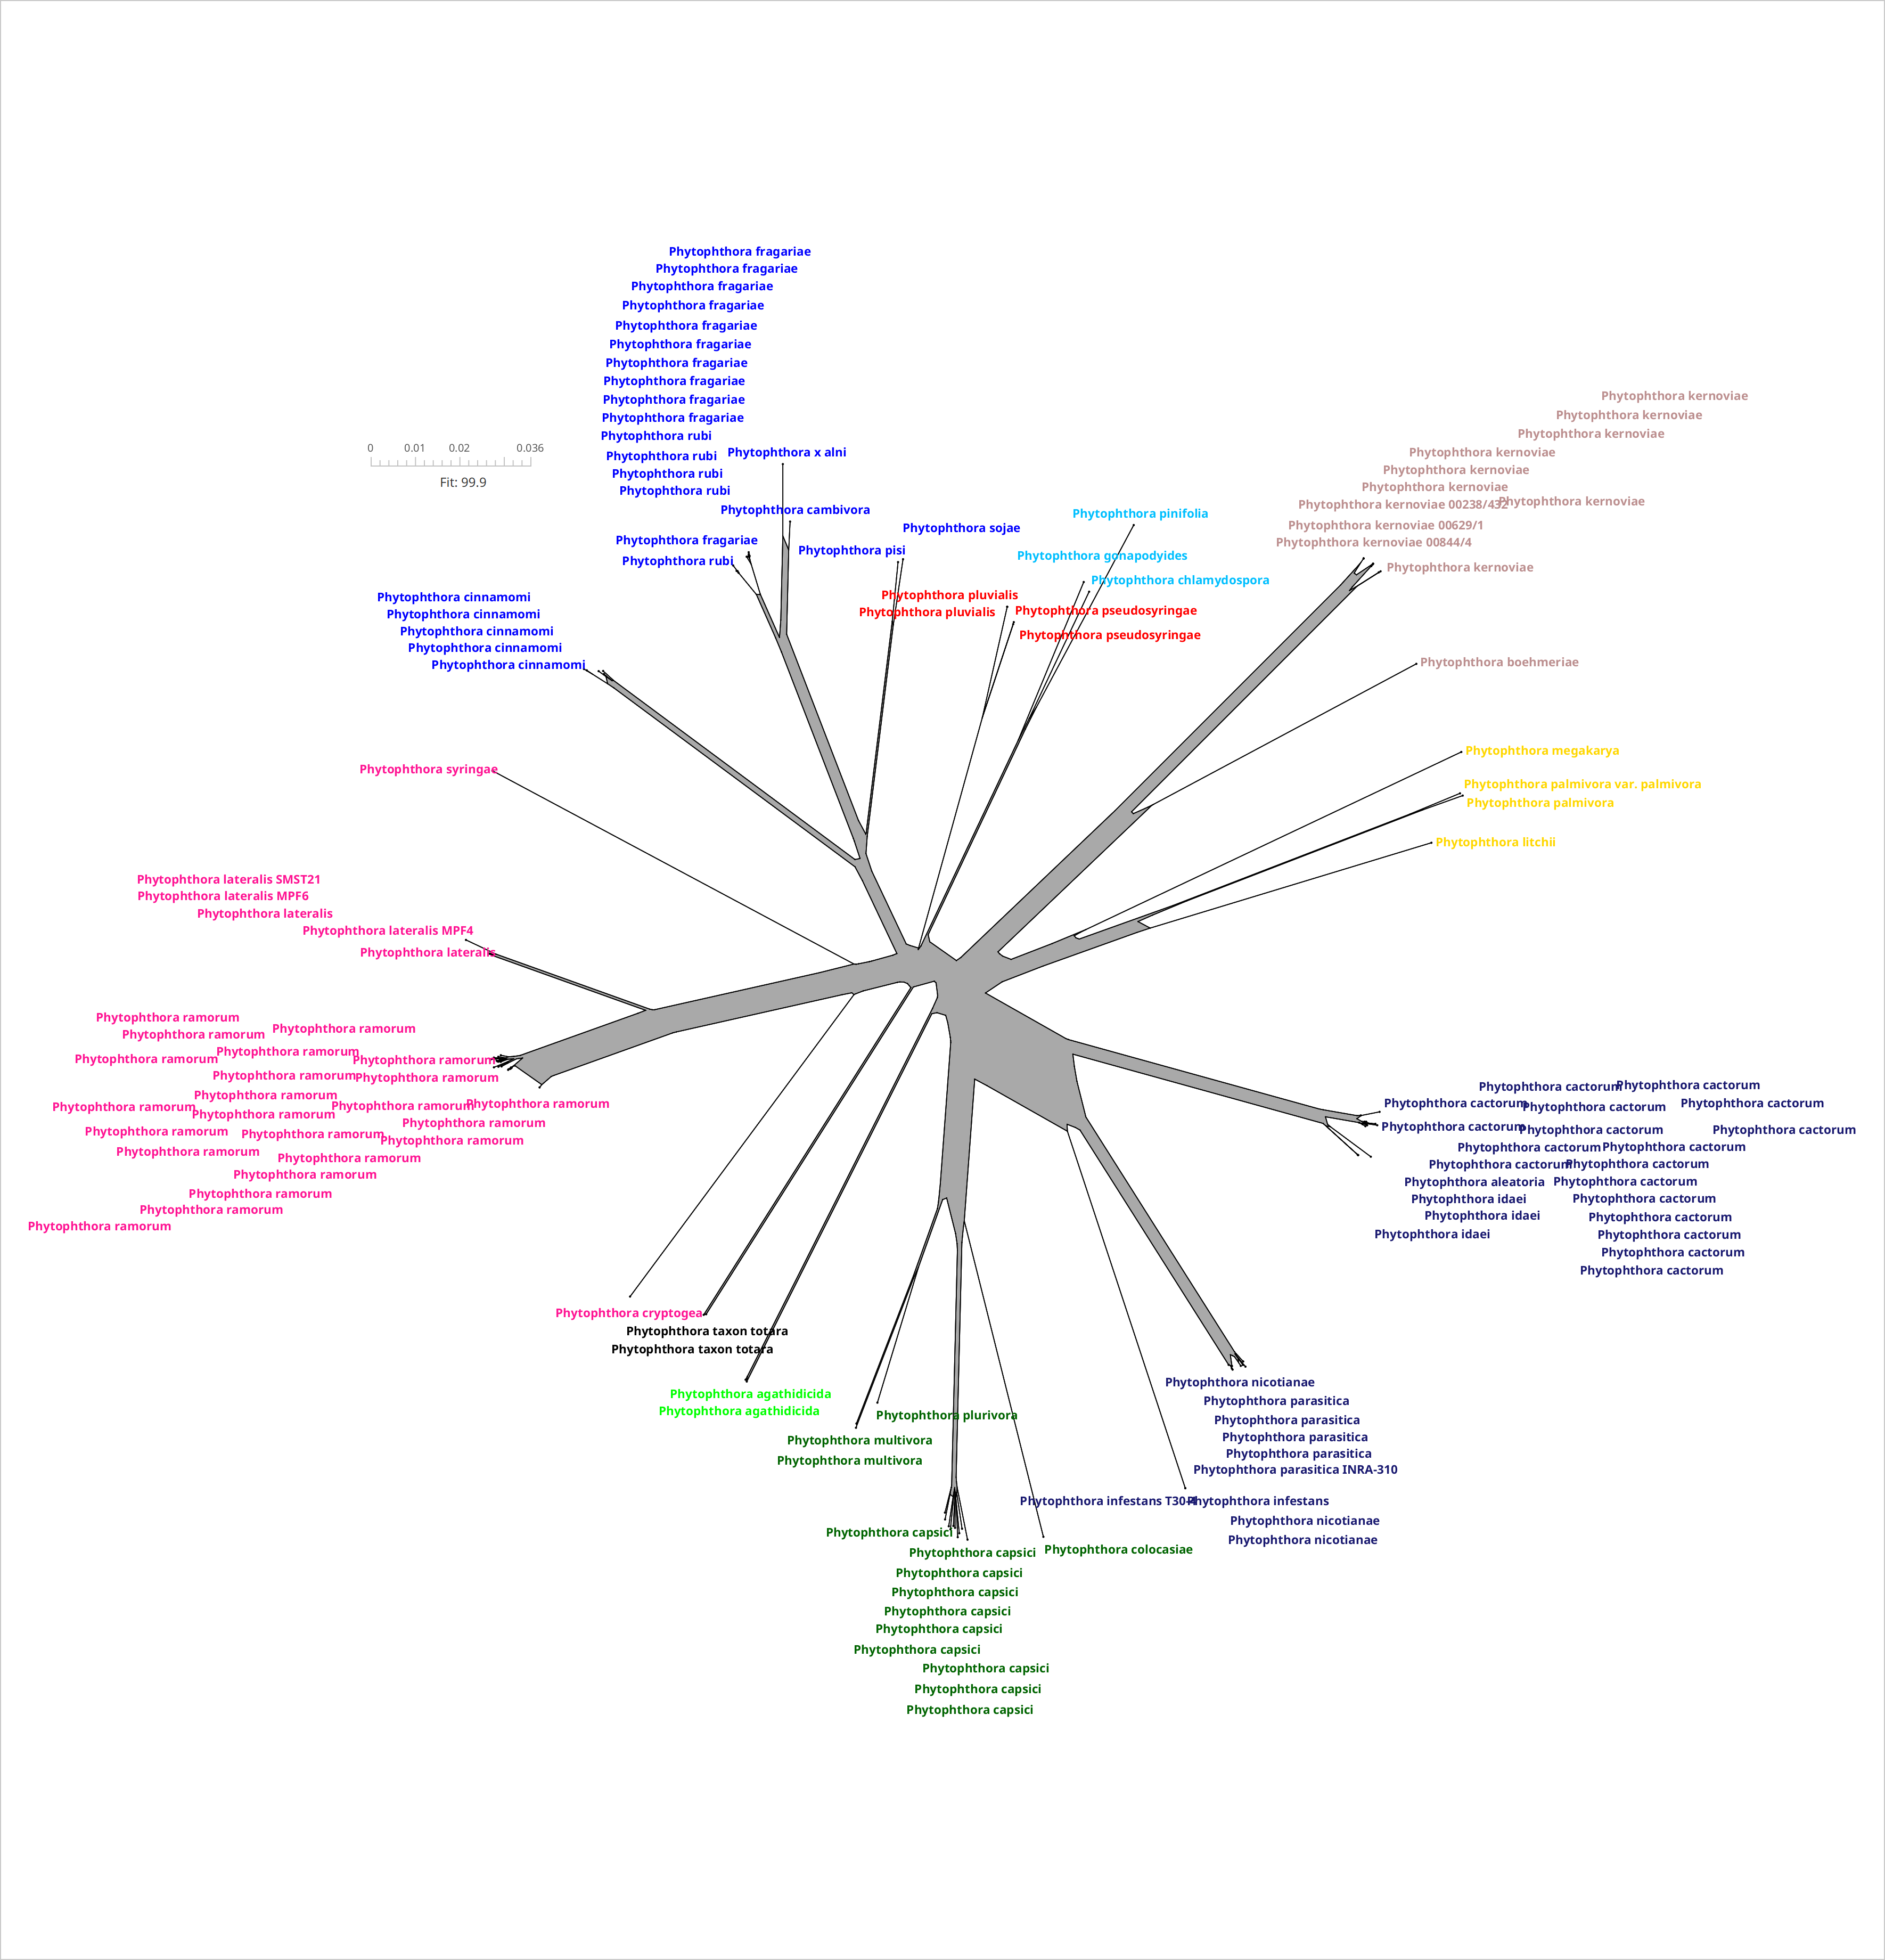
\includegraphics[width=1.0\textwidth]{figures/mashtree_mandal_outline_k21_s2000.png}
  \caption[Phylogenetic outline based on distances of dataset \textbf{A}
  calculated with \texttt{mashtree}]{Phylogenetic outline based on distances of
  dataset \textbf{A} calculated with
  \texttt{mashtree}
  \cite{ondovMashFastGenome2016,katzMashtreeRapidComparison2019}. Taxa are
  colored according to clade membership
  \cite{abadPhytophthoraTaxonomicPhylogenetic2023a}.}
  \label{fig:mandalMashOutline}
\end{figure}

The phyloegenetic outline that was calculated using the FracMinHash distance for
dataset \textbf{A} is depicted in Figure~\ref{fig:mandalFmhdistTree}. Again,
clusters are well defined and in line with literature, the same holds true for
the subclades
\cite{abadPhytophthoraTaxonomicPhylogenetic2023a,yangExpandedPhylogenyGenus2017}.

\begin{figure}
  \centering
  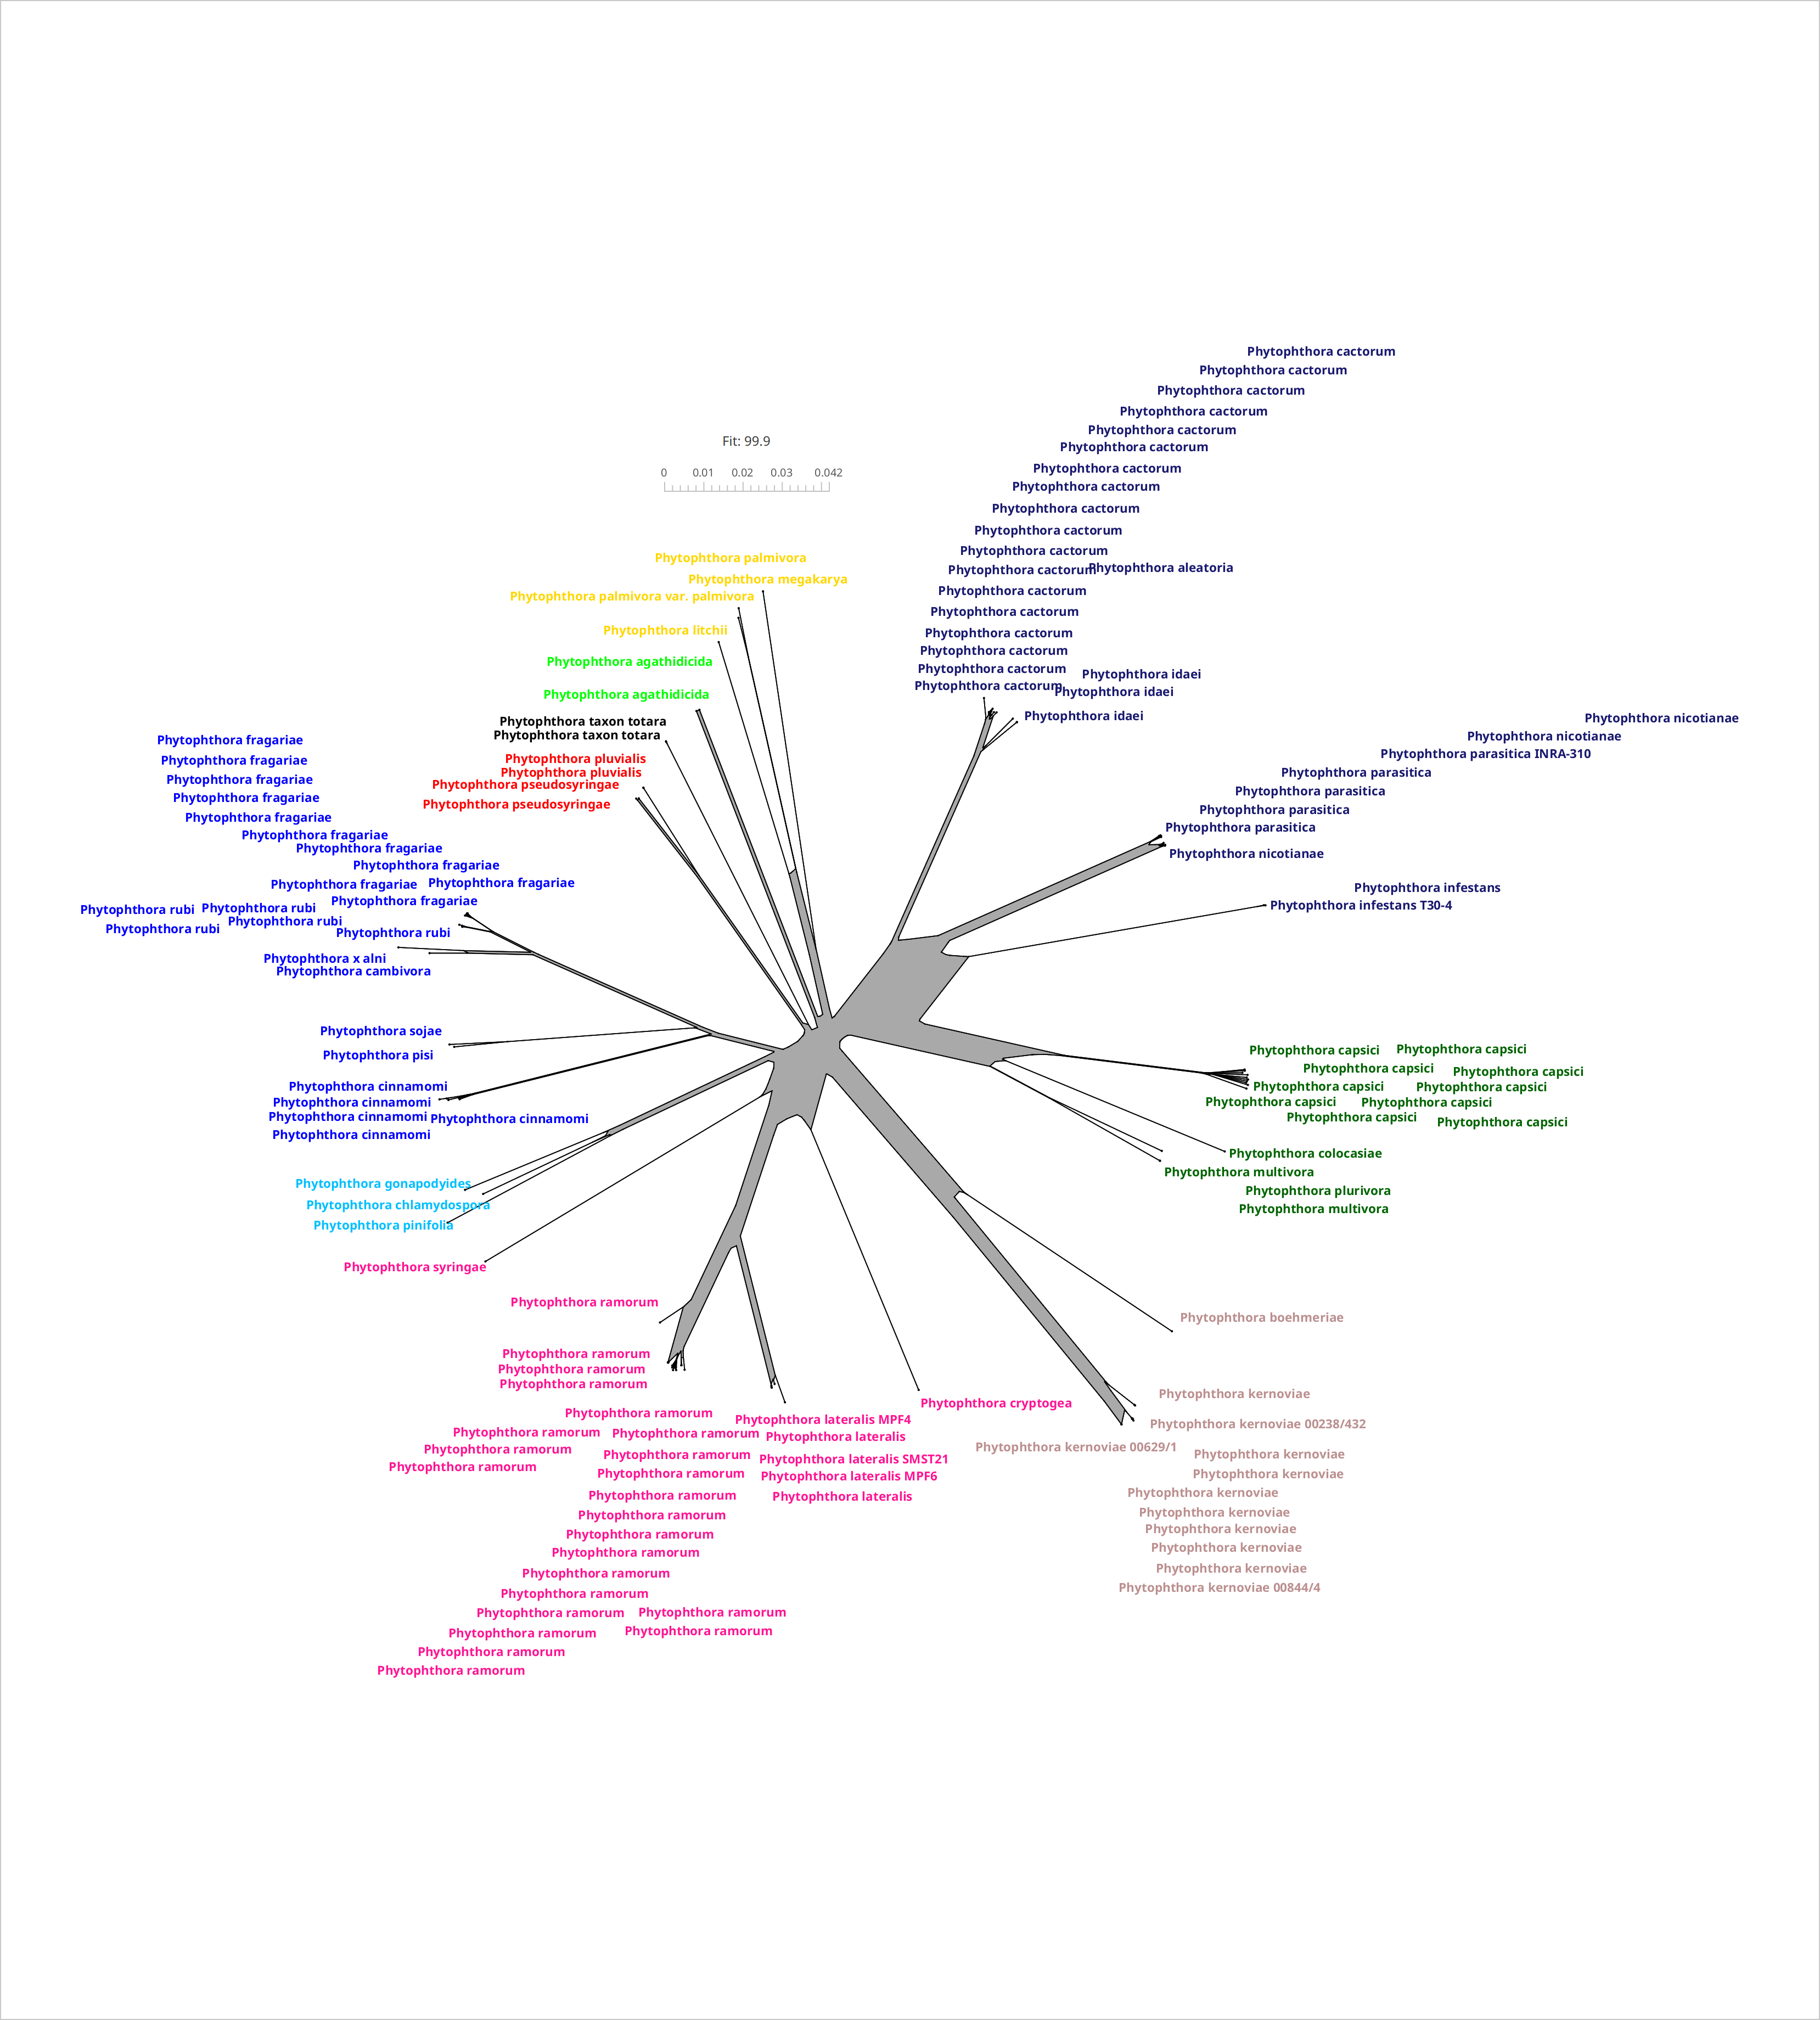
\includegraphics[width=1.0\textwidth]{figures/fmhdist_mandal_outline_k21_s2000.png}
  \caption[Phylogenetic outline based on distances of dataset \textbf{A}
  calculated with \texttt{fmhdist}]{Phylogenetic outline based on distances of
  dataset \textbf{A} calculated with \texttt{fmhdist}. Taxa are colored according to
  clade membership \cite{abadPhytophthoraTaxonomicPhylogenetic2023a}.}
  \label{fig:mandalFmhdistOutline}
\end{figure}

Comparing the outlines and the underlying splits, one noteable difference is the
relationship betwen clades 8 and 10. The \texttt{fmhdist} distances provide a
split $S= \{1, 2, 3, 4, 5\} | \{6, 7, 8, 10\}$ and $S= \{1, 2, 3, 4, 5, 6, 7\} |
\{8, 10\}$. Although those clade clusters are in line with literature
\cite{yangExpandedPhylogenyGenus2017,abadPhytophthoraTaxonomicPhylogenetic2023a},
they are not present when using the \texttt{mashtree} distances.


\section{Split differences are measurable}
As seen in Table~\ref{ta:splitDifferences}, the splits generated from the
\texttt{mashtree} distances differ from the splits generated by
\texttt{fmhdist}, i.e. there are splits in the former that are not in the latter
and vice versa. Compared to the difference between the three different distance
metrics implemented in \texttt{fmhdist}, we can observe that the number of
split differences is much smaller and thus the total weight associated with
those differences. The Robinson-Foulds distance $D_{RF}$ is very similar in all
three comparisons.

\begin{table}[]
  \centering
  \begin{tabular}{@{}lrrr@{}}
    \toprule
    &  \textbf{I} & \textbf{II} & \textbf{III} \\
    \midrule
  $\sum_{s \in \Sigma_A}{\omega(s)}$           & 1.3064                     & 1.3064                              & 1.3064                         \\
  $\sum_{s \in \Sigma_B}{\omega(s)}$           & 1.4321                     & 1.2990                              & 1.4339                         \\
  $\sum_{s \in \Sigma_A / \Sigma_B}{\omega(s)}$ & 0.1059                    & 0.0174                              & 0.0299                      \\
  $\sum_{s \in \Sigma_B / \Sigma_A}{\omega(s)}$ & 0.1061                    & 0.0142                             & 0.0335                       \\
  $|\Sigma_A / \Sigma_B|$                       & 103                       & 31                                 & 54                                        \\
  $|\Sigma_B / \Sigma_A|$                       & 75                        & 27                                 & 48                                        \\
  $D_{RF}(\Sigma_A, \Sigma_B)$                 & 149.0                       & 161.0                                & 160.5         \\
  \bottomrule                           
  \end{tabular}
  \caption[Comparison of different sets of splits based on different distance
  calculations of dataset \textbf{A}]{Comparison of different sets of splits
  based on different distance calculations of dataset \textbf{A}. \textbf{I} is
  the comparison of \texttt{fmhdist} against \texttt{mashtreee}. \textbf{II} is
  the comparison of \texttt{fmhdist} against \texttt{fmhdist containment}.
  \textbf{III} is the comparison of \texttt{fmhdist} against \texttt{fmhdist
  mash}.}
  \label{ta:splitDifferences}
\end{table}


\section{Impact of parameter choices}
\subsection*{Impact of the choice of $k$ and $s$}
At the typical $k$-mer size of $k=21$
\cite{mandalComparativeGenomeAnalysis2022,ondovMashFastGenome2016,irberLightweightCompositionalAnalysis2022},
the method performs well as described above. Using $k \in \{19, 20, 22, 25\}$
does not change the produced outline substantially. This is also backed by the
calculated sum of split weights and the differences therein. Comparing $k=21$
with $k=25$ indicates a very small difference in the total weight ($1.3064$ vs
$1.2413$), a difference that is smaller than comparing Mash and FracMinHash.
Extreme values, such as $k=10$ break the clusters such that species are not
clustered accoding to clade membership anymore. Using such a small $k$ leads to
a very low total weight of splits ($0.3374$) and in general unusual outlines.

Different values of $s$ change the sketch size. Using $s=2000$, the sketch sizes
range from $17397$ to $66726$ with a median at $24906$. Using $s=4000$, the
sketch sizes range from $8738$ to $33504$ with a median at $12423$. The sketch
sizes are clearly halved which is to be expected when doubling $s$.

The impact of changing $s$ in the given range is small in terms of splits and
outlines. Changing $s$ rotates or mirrors parts of the outline, introduces
splits and removes others, but all of those differences have minor impact on
interpreting the generated outline. This is also indicated by the differences in
split weight, the total weight of splits for the four different variants of $s$
is in the interval $[1.3064, 1.3165]$. The weight of split differences is the
range $[0.0419, 0.0805]$.

\subsection*{Impact of the choice of hash function}
While all hash functions are capable of hashing tens of millions keys of size
$21$ per second, the runtime varies a lot when observered in detail
(Table~\ref{ta:hashbenchmark}). The best runtime for keys of size $21$ was
achieved with the two variants of FarmHash, followed by WyHash and CityHash. The
hash function used by \texttt{mash} and \texttt{sourmash}, MurMur3
\cite{ondovMashFastGenome2016,irberLightweightCompositionalAnalysis2022}, only
achieves medium speed in comparison to the other hash functions.  

\begin{table}[]
  \centering
  \begin{tabular}{@{}lr@{}}
  \toprule
  \textbf{Hash Function }& \textbf{Throughput (ops/s)}                      \\
  \midrule
  CityHash      & 53502048.778 ± 4483465.863   \\
  FarmHash 1.0  & 55008714.492 ± 2363256.004   \\
  FarmHash 1.1  & 54678293.943 ±  482133.235   \\
  MetroHash     & 51132334.855 ±  307903.868   \\
  MurMur 3      & 36500708.446 ±  497774.958   \\
  WyHash        & 54259034.831 ± 1327599.078   \\
  XX128         & 22684338.104 ±   98278.977   \\
  XX3           & 27170615.109 ±  220725.087   \\
  XX64          & 44799765.447 ± 1091771.572  \\
  \bottomrule
  \end{tabular}
  \caption{Results of the hash function benchmark for keys of size $21$.}
  \label{ta:hashbenchmark}
  \end{table}


\section{Sketches of mtDNA are very small}
Outlines and trees generated from the FracMinHash distances for dataset
\textbf{B} with $s=1000$ are not usable. Most of the distances are 0, thus edge
lengths are too short to separate taxa in any meaningful way. The smallest
sketch has $29$ hashes, the largest $54$. The same behaviour can be observed
when sketching viral genomes stored in NCBI. Using smaller values for $s$
creates clusters that resemble the clade membership well
\cite{abadPhytophthoraTaxonomicPhylogenetic2023a,yangExpandedPhylogenyGenus2017}.
The outlines from dataset \textbf{B} with $s=100$ are depicted in
Figure~\ref{fig:winkworthTree}. Here, sketch sizes range from $333$ to $454$.
Comparing the trees and outlines for $s=1$ values to published phylogenies
\cite{abadPhytophthoraTaxonomicPhylogenetic2023a,yangExpandedPhylogenyGenus2017},
we can observe that several relationships between clades are not depicted, e.g.
the clades 1, 2 and 4 or the clades 8 and 10 can only be clustered when adding
more clades.


The tree published in \cite{winkworthComparativeAnalysesComplete2022} has the
following topology:

\texttt{((((((((((1, 16), 4), 3), (2, (5, 12)), 15), 6),
7), 8), (9, 10), \textit{Nothophytophthora sp.}), \textit{Phytopythium vexans}),
\textit{Phytium ultimum})}

The FracMinHash tree as depicted in Figure~\ref{fig:winkworthTree} has the topology

\texttt{(((((((((((5, 12), 15b), 1), (3, 4)), (8, (6, (7, 2)))), (9, 10)), 16),
15a), \textit{Nothophytophthora sp.}), \textit{Phytopythium
vexans}), \textit{Phytium ultimum})}


There are so many differences in the trees that it is easier to list shared
aspects. Noteably, the clustering of clades 5 and 12, and 9 and 10 as well as
the placement of the outgroups\textit{Phytium ultimum}, \textit{Phytopythium
vexans} and \textit{Nothophytophthora sp.} are shared between the two trees.

\begin{figure}
  \centering
  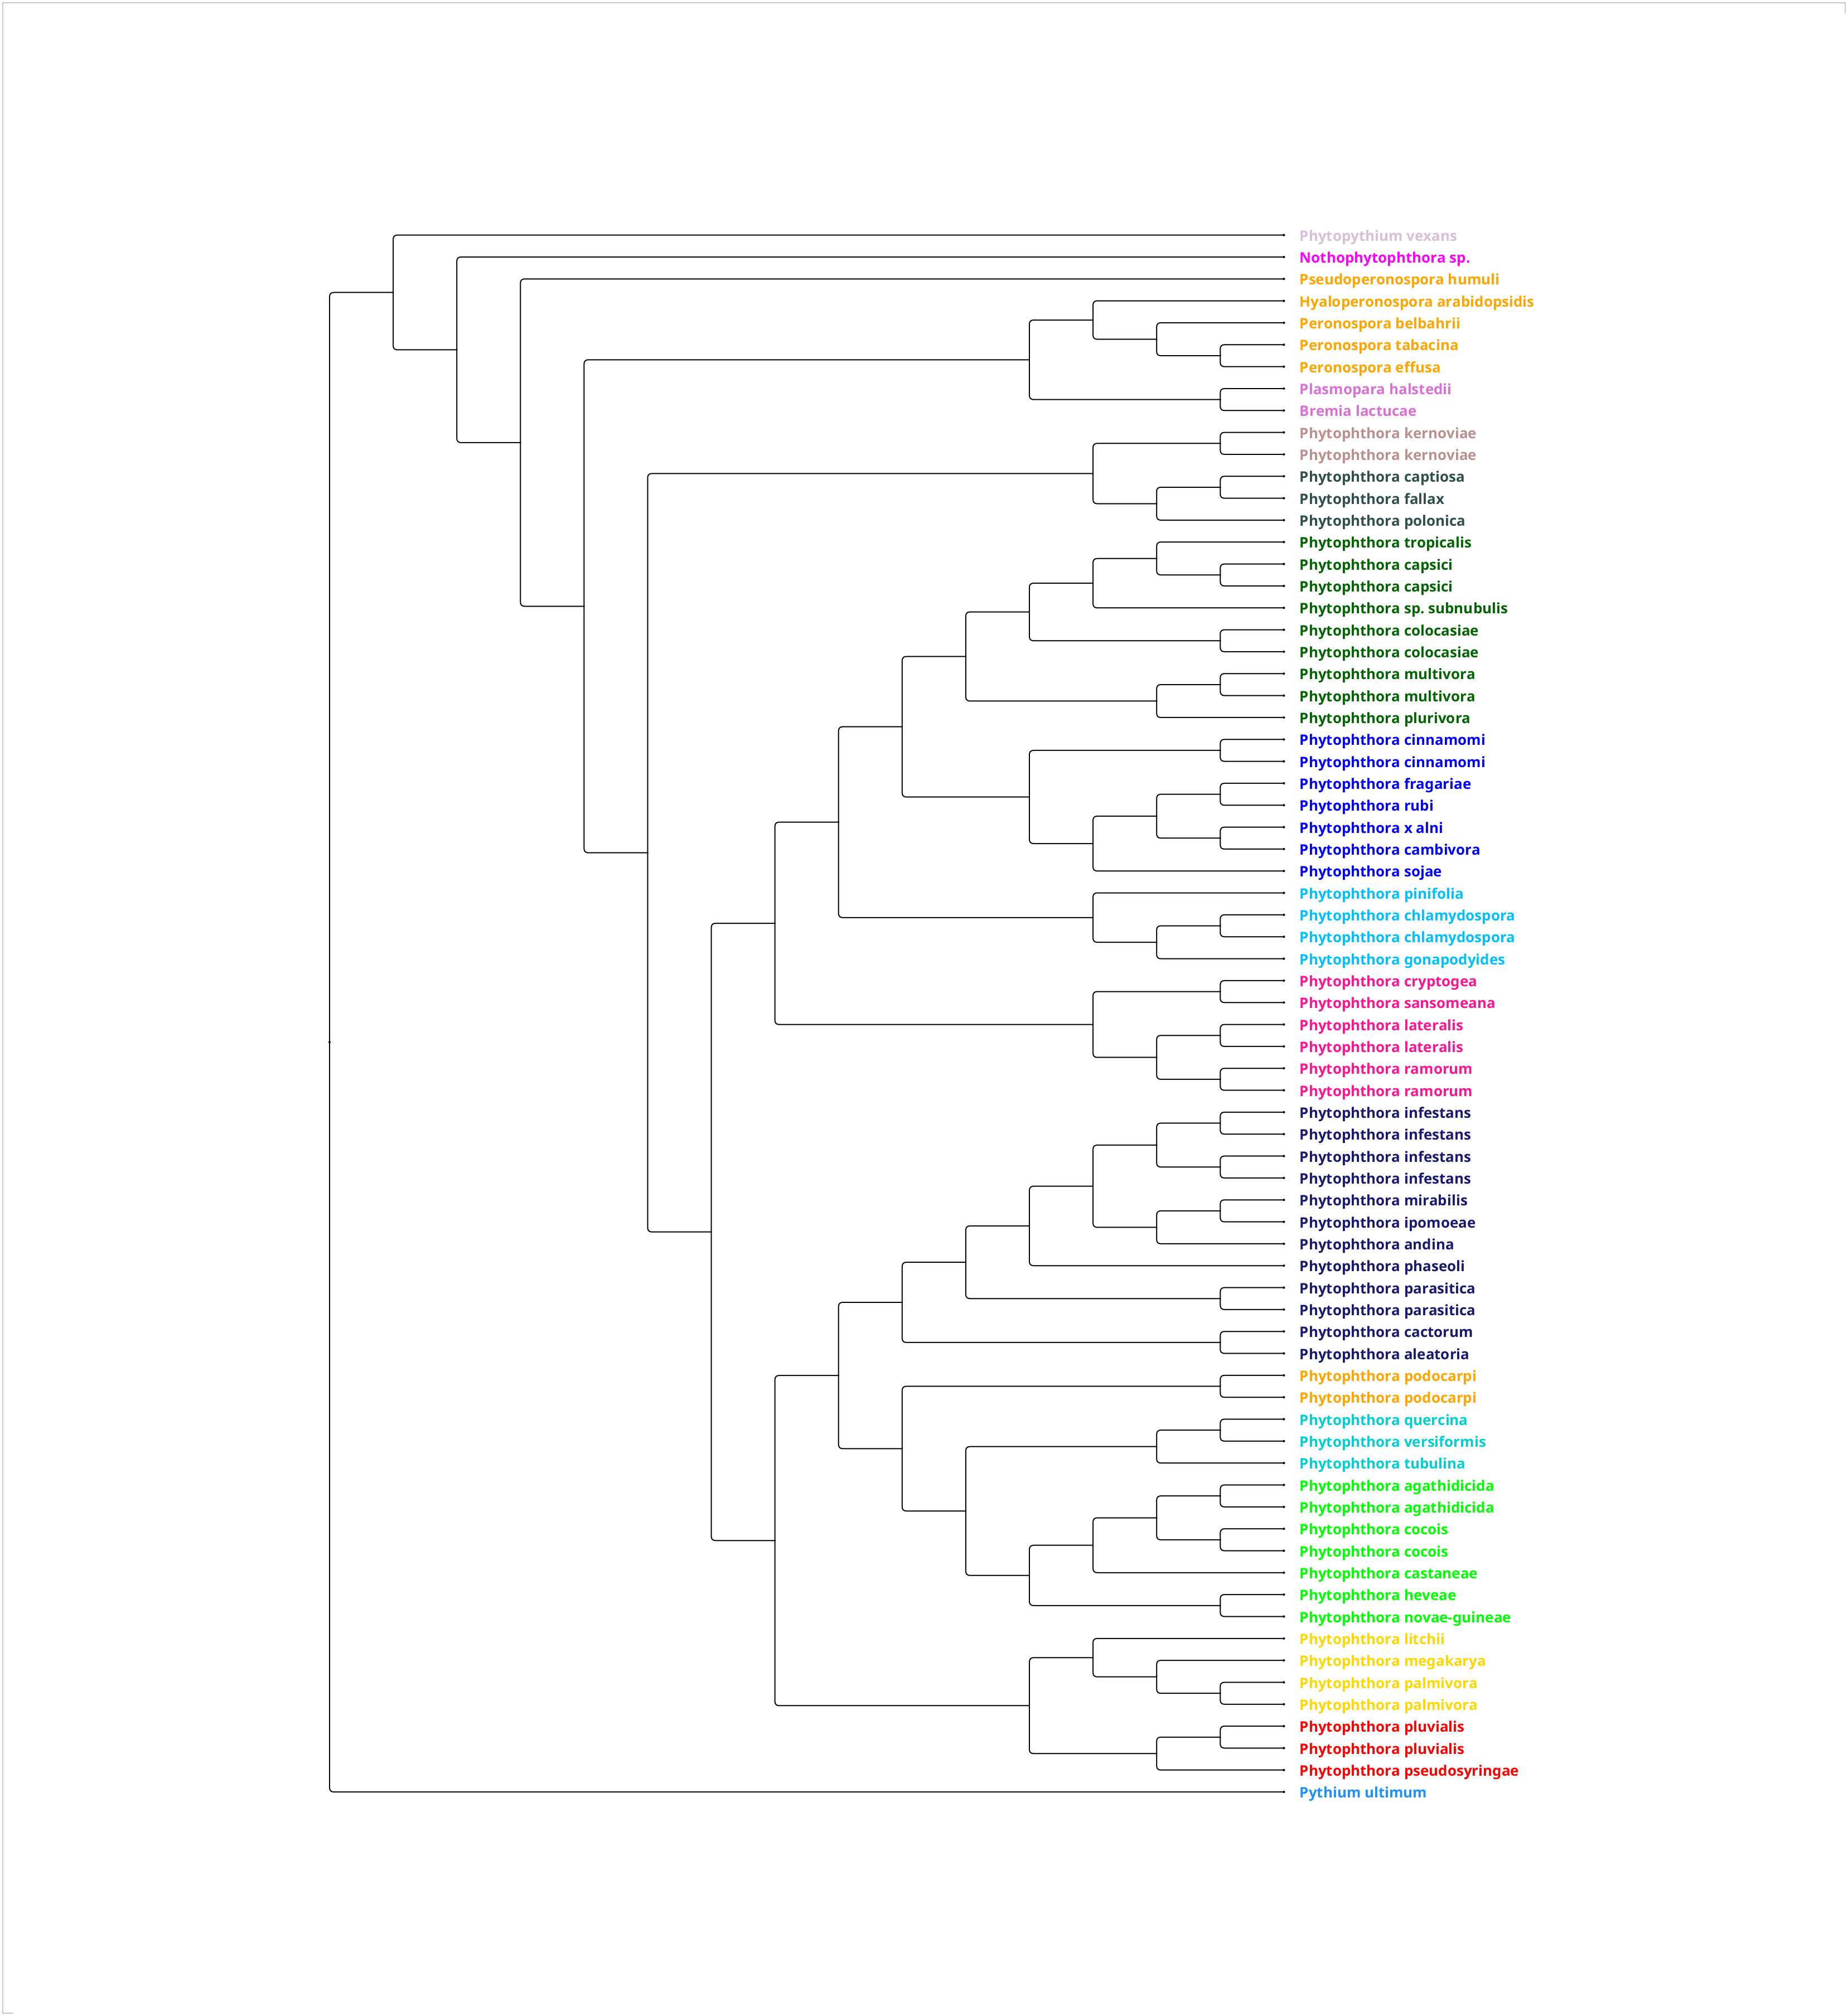
\includegraphics[width=0.80\textwidth]{figures/fmhdist_winkworth_tree_k21_s100.png}
  \caption[Phylogenetic tree based on distances of dataset \textbf{B} calculated
  with \texttt{fmhdist}]{Phylogenetic tree based on distances of dataset
  \textbf{B} calculated with \texttt{fmhdist} using $k=21$ and $s=100$. Taxa are
  colored according to clade membership
  \cite{abadPhytophthoraTaxonomicPhylogenetic2023a,winkworthComparativeAnalysesComplete2022}.
  The tree is rooted with \textit{Phytium ultimum} as outgroup.}
  \label{fig:winkworthTree}
\end{figure}

\section{FracMinHash estimates distances for distantly related genomes}
\sectionmark{Distantly related Genomes}
The different outlines based on the \texttt{mashtree} and \texttt{fmhdist}
($s=2000$) distances of dataset \textbf{C}, respectively, are depicted in
Figure~\ref{fig:avocadoOutlineComparison}. Of interest is the placement of the
query genomes: the bacterial queries are very clearly separated from the all
\textit{Phytophthora} reference genomes in both outlines. This is not true for
the two fungal queries, they are placed in between the \textit{Phytophthora}
reference genomes in the \texttt{fmhdist} variant but also as outliers in the
\texttt{mashtree} variant.

\begin{figure}
  %\fontsize{8}{10}
  %\selectfont
  \centering
  \begin{subfigure}{0.49\textwidth}
    %\includesvg[width=1.0\textwidth]{figures/fmhdist_avodado4-1_k21_s2000.svg}
    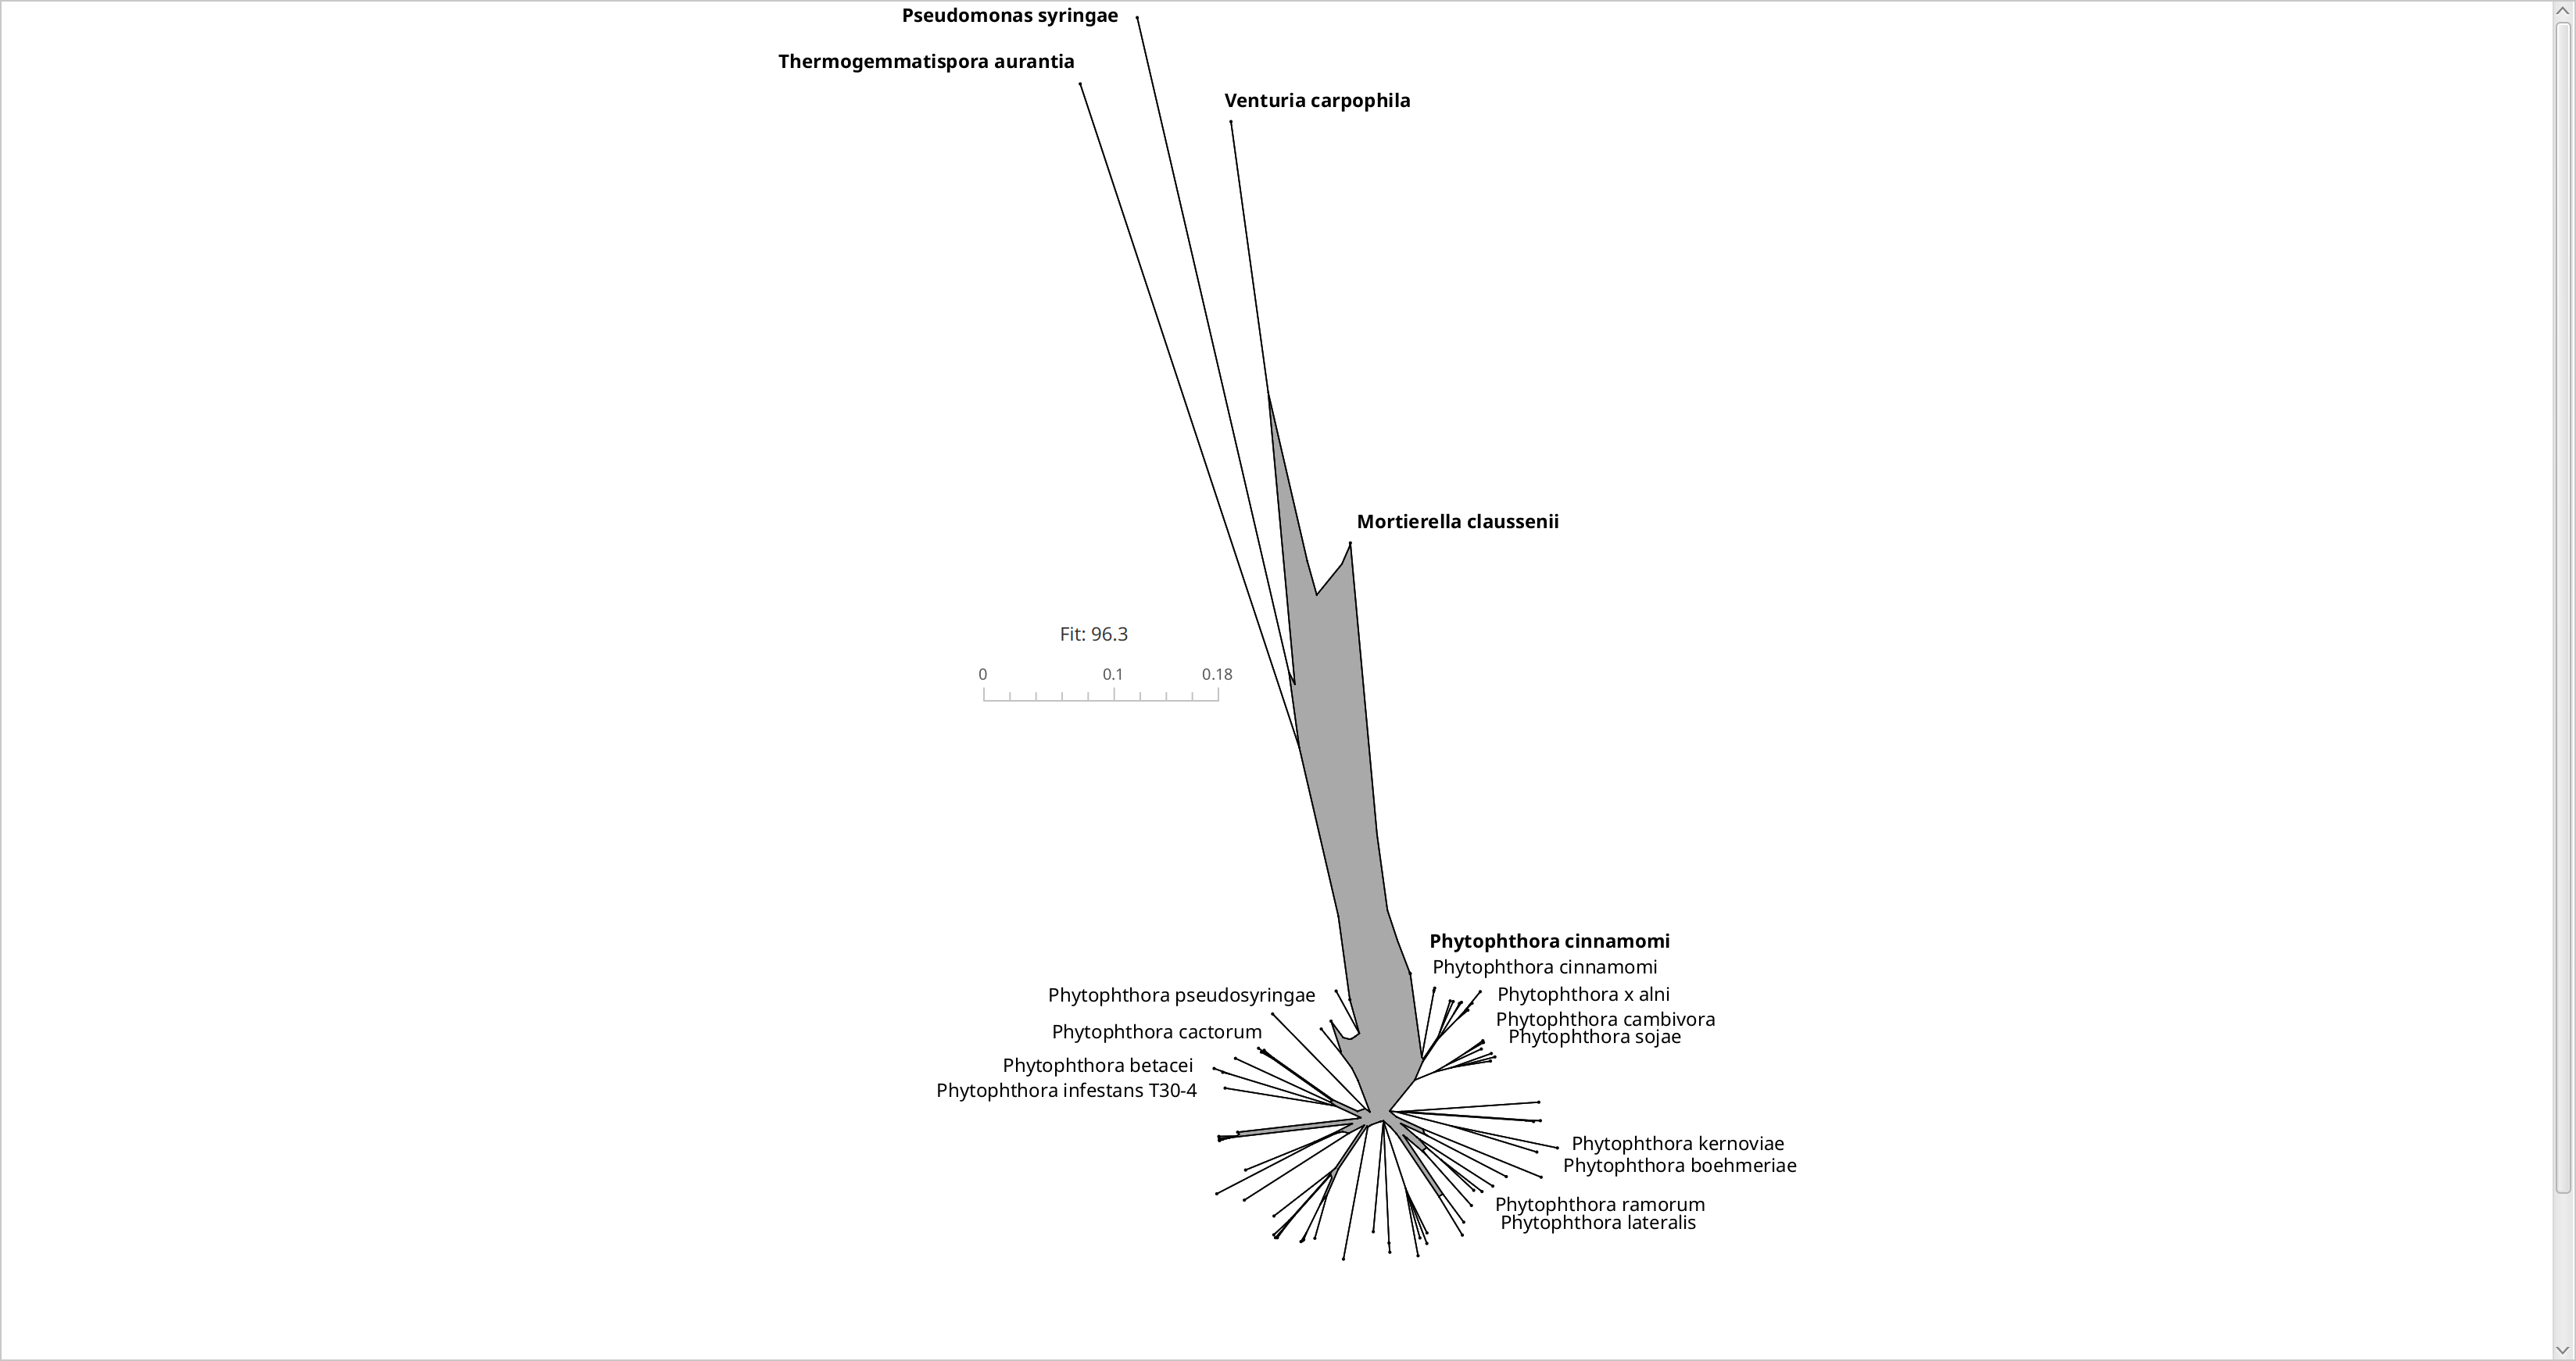
\includegraphics[width=1.0\textwidth]{figures/mashtree_avocado4-1_k21_s2000.png}
  \end{subfigure}
  \begin{subfigure}{0.49\textwidth}
    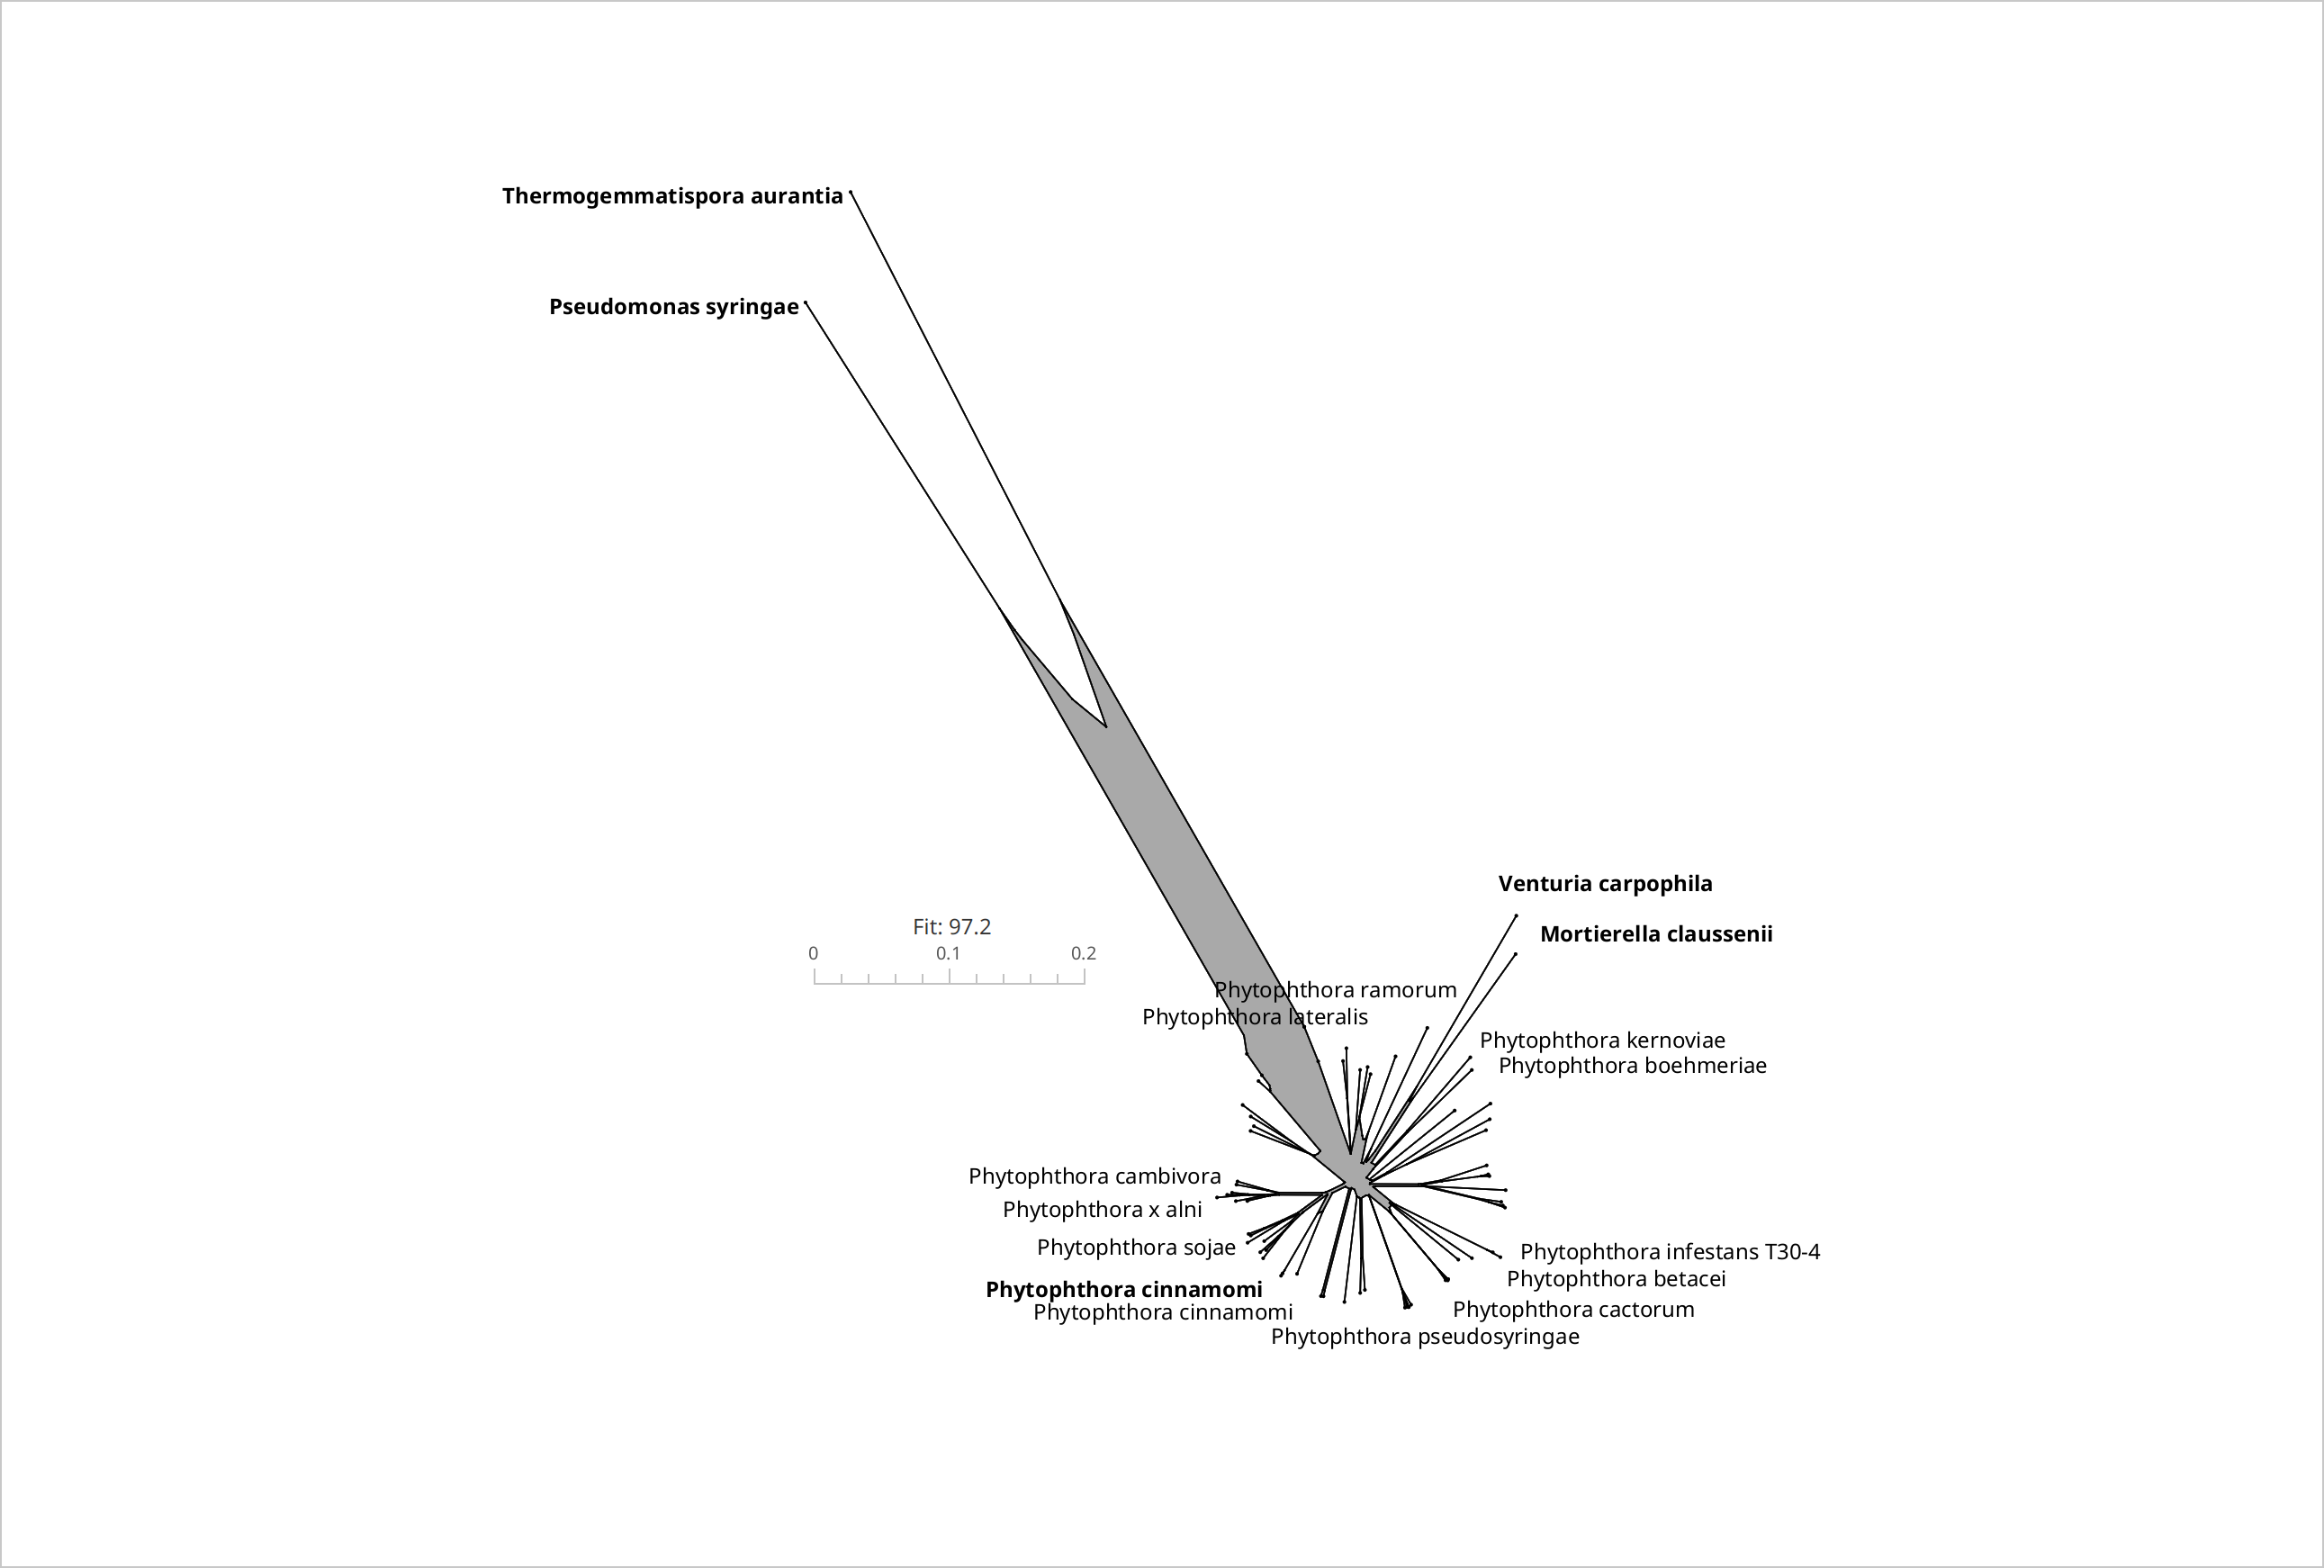
\includegraphics[width=1.0\textwidth]{figures/fmhdist_avocado4-1_k21_s2000.png}
  \end{subfigure}
  \caption[Phylogenetic outlines of dataset \textbf{C}]{Phylogenetic outlines of
  dataset \textbf{C}, query sequences are formatted bold. To increase
  readability, only a small subset of reference labels are displayed. Left is
  the outline based on \texttt{mashtree} distances, right is the outline based
  on \texttt{fmhdist} distances.}
  \label{fig:avocadoOutlineComparison}
\end{figure}

This behaviour can obviously also be observed when comparing the distances of
the five queries and the \textit{Phytophthora infestans} reference directly
(Table~\ref{ta:avocadoDistance}). All distances involving the bacterial queries
are $1.0$.

The Mash distance for \textit{Venturia carpophila} is $1.0$ for the comparison
to the bacterial queries, \textit{Phytophthora infestans} and
\textit{Phytophthora cinnamomi}. The distance is $0.3726$ for the comparison
with the other fungal query, \textit{Mortierella claussenii}. This query
sequence, in turn, does have low distances of $0.3290$ and $0.4056$ to
\textit{Phytophthora cinnamomi} and \textit{Phytophthora infestans},
respectively.

For FracMinHash, we can see that both fungal queries have a distance below 1 to
the two \textit{Phytophthora} genomes.


% Please add the following required packages to your document preamble:
% \usepackage{booktabs}
\begin{table}[]
  \centering
  \begin{tabular}{@{}llrrrrrr@{}}
  \toprule
              &                      & \textbf{F1} & \textbf{F2} & \textbf{B1} & \textbf{B2} & \textbf{P1} & \textbf{P2} \\ \midrule
  \textbf{F1} & \textbf{Mash}        & 0.0000      & 0.3726      & 1.0000      & 1.0000      & 0.3290      & 0.4056      \\
  \textbf{}   & \textbf{FracMinHash} & 0.0000      & 0.3024      & 1.0000      & 1.0000      & 0.3010      & 0.3101      \\ \midrule
  \textbf{F2} & \textbf{Mash}        & 0.3726      & 0.0000      & 1.0000      & 1.0000      & 1.0000      & 1.0000      \\
  \textbf{}   & \textbf{FracMinHash} & 0.3024      & 0.0000      & 1.0000      & 1.0000      & 0.3278      & 0.3338      \\ \midrule
  \textbf{B1} & \textbf{Mash}        & 1.0000      & 1.0000      & 0.0000      & 1.0000      & 1.0000      & 1.0000      \\
  \textbf{}   & \textbf{FracMinHash} & 1.0000      & 1.0000      & 0.0000      & 1.0000      & 1.0000      & 1.0000      \\ \midrule
  \textbf{B2} & \textbf{Mash}        & 1.0000      & 1.0000      & 1.0000      & 0.0000      & 1.0000      & 1.0000      \\
  \textbf{}   & \textbf{FracMinHash} & 1.0000      & 1.0000      & 1.0000      & 0.0000      & 1.0000      & 1.0000      \\ \midrule
  \textbf{P1} & \textbf{Mash}        & 0.3290      & 1.0000      & 1.0000      & 1.0000      & 0.0000      & 0.2470      \\
  \textbf{}   & \textbf{FracMinHash} & 0.3010      & 0.3278      & 1.0000      & 1.0000      & 0.0000      & 0.2252      \\ \midrule
  \textbf{P2} & \textbf{Mash}        & 0.4056      & 1.0000      & 1.0000      & 1.0000      & 0.2470      & 0.0000      \\
  \textbf{}   & \textbf{FracMinHash} & 0.3101      & 0.3338      & 1.0000      & 1.0000      & 0.2252      & 0.0000      \\ \bottomrule
  \end{tabular}
  \caption[Distance estimation for selected species in dataset \textbf{C}
  calculated with \texttt{mashtree} and \texttt{fmhdist}]{Distance estimation
  for selected species in dataset \textbf{C} calculated with \texttt{mashtree}
  with default settings and \texttt{fmhdist} with $k=21$, $s=2000$, FarmHash and
  random seed $rs=42$ for \textit{Mortierella claussenii} (F1), \textit{Venturia
  carpophila} (F2), \textit{Pseudomonas syringae} (B1),
  \textit{Thermogemmatispora aurantia} (B2), \textit{Phytophthora cinnamomi}
  (P1) and \textit{Phytophthora infestans} (P2) of dataset C}
  \label{ta:avocadoDistance}
\end{table}

This is in line with the empty intersections produced by both methods when
comparing sketches. Using different random seeds to sketch dataset \textbf{C}
and counting the occurrence of empty intersections of the resulting sketches, we
can see that FracMinHash produces non-empty intersections more often than Mash
(Table~\ref{ta:avodadoIntersections}). This doesn't change when scaling
FracMinHash such that the sketch sizes of particular query genomes are close to
$10000$.


% Please add the following required packages to your document preamble:
% \usepackage{booktabs}
\begin{table}[]
  \centering
  \begin{tabular}{@{}llrrrrrr@{}}
  \toprule
  \textbf{}   & \textbf{}                      & \textbf{F1} & \textbf{F2} & \textbf{B1} & \textbf{B2} & \textbf{P1} & \textbf{P2} \\ \midrule
  \textbf{F1} & \textbf{Mash}                  & 0           & 1           & 3           & 1           & 0           & 1           \\
  \textbf{}   & \textbf{FracMinHash, $s=2000$} & 0           & 0           & 4           & 3           & 0           & 0           \\
  \textbf{}   & \textbf{FracMinHash, $s=500$}  & 0           & 0           & 3           & 0           & 0           & 0           \\
  \textbf{}   & \textbf{FracMinHash, $s=3500$} & 0           & 0           & 4           & 4           & 0           & 0           \\ \midrule
  \textbf{F2} & \textbf{Mash}                  & 1           & 0           & 5           & 4           & 4           & 1           \\
  \textbf{}   & \textbf{FracMinHash, $s=2000$} & 0           & 0           & 4           & 5           & 0           & 0           \\
  \textbf{}   & \textbf{FracMinHash, $s=500$}  & 0           & 0           & 1           & 2           & 0           & 0           \\
  \textbf{}   & \textbf{FracMinHash, $s=3500$} & 0           & 0           & 4           & 5           & 0           & 0           \\ \midrule
  \textbf{B1} & \textbf{Mash}                  & 3           & 5           & 0           & 2           & 5           & 4           \\
              & \textbf{FracMinHash, $s=2000$} & 4           & 4           & 0           & 3           & 4           & 3           \\
              & \textbf{FracMinHash, $s=500$}  & 3           & 1           & 0           & 2           & 2           & 0           \\
              & \textbf{FracMinHash, $s=3500$} & 4           & 4           & 0           & 3           & 4           & 4           \\ \midrule
  \textbf{B2} & \textbf{Mash}                  & 1           & 4           & 2           & 0           & 4           & 3           \\
  \textbf{}   & \textbf{FracMinHash, $s=2000$} & 3           & 5           & 3           & 0           & 2           & 3           \\
  \textbf{}   & \textbf{FracMinHash, $s=500$}  & 0           & 2           & 2           & 0           & 1           & 1           \\
  \textbf{}   & \textbf{FracMinHash, $s=3500$} & 4           & 5           & 3           & 0           & 4           & 3           \\ \midrule
  \textbf{P1} & \textbf{Mash}                  & 0           & 4           & 5           & 4           & 0           & 0           \\
  \textbf{}   & \textbf{FracMinHash, $s=2000$} & 0           & 0           & 4           & 2           & 0           & 0           \\
  \textbf{}   & \textbf{FracMinHash, $s=500$}  & 0           & 0           & 2           & 1           & 0           & 0           \\
  \textbf{}   & \textbf{FracMinHash, $s=3500$} & 0           & 0           & 4           & 4           & 0           & 0           \\ \midrule
  \textbf{P2} & \textbf{Mash}                  & 1           & 1           & 4           & 3           & 0           & 0           \\
  \textbf{}   & \textbf{FracMinHash, $s=2000$} & 0           & 0           & 3           & 3           & 0           & 0           \\
  \textbf{}   & \textbf{FracMinHash, $s=500$}  & 0           & 0           & 0           & 1           & 0           & 0           \\
              & \textbf{FracMinHash, $s=3500$} & 0           & 0           & 4           & 3           & 0           & 0           \\ \bottomrule
  \end{tabular}
  \caption[Comparison of frequencies of empty intersections in the numerator of
  the Mash and FracMinHash Jaccard estimation, respectively, given 5 different
  random seeds]{Comparison of frequencies of empty intersections in the
  numerator of the Mash and FracMinHash Jaccard estimation, respectively, given
  5 different random seeds. Sketches were generated with \texttt{mashtree} with
  the default settings and \texttt{fmhdist} with $k=21$, $s$ as stated in the
  table and FarmHash for \textit{Mortierella claussenii} (F1), \textit{Venturia
  carpophila} (F2), \textit{Pseudomonas syringae} (B1),
  \textit{Thermogemmatispora aurantia} (B2), \textit{Phytophthora cinnamomi}
  (P1) and \textit{Phytophthora infestans} (P2) of dataset \textbf{C}.}
  \label{ta:avodadoIntersections}
\end{table}

The ANI values for the six genomes in question do not provide a good baseline to
compare against as they are not intended to compare species above the rank of
genus \cite{leeOrthoANIImprovedAlgorithm2016}. This is reflected by the actual
values obtained from \texttt{OrthoANI}, they range from $0.61$ to $0.65$ for all
15 comparisons.

The AAI values (Table~\ref{ta:avodadoAAI}) are more useful for the comparison of
distantly related genomes \cite{rodriguez-rEnveomicsCollectionToolbox2016}, but
still don't go below $0.3$. We can see clear spikes for the identity values of
\textit{Phytophthora infestans} against \textit{Phytophthora cinnamomi} and
\textit{Mortierella claussenii} against \textit{Venturia carpophila}, indicating
a closer evolutionary relationship of those.

\begin{table}[]
  \centering
  \begin{tabular}{@{}lrrrrrr@{}}
  \toprule
              & \textbf{F1} & \textbf{F2} & \textbf{B1} & \textbf{B2} & \textbf{P1} & \textbf{P2} \\ \midrule
  \textbf{F1} & 1.0000      & 0.4152      & 0.3407      & 0.3401      & 0.3922      & 0.3916      \\
  \textbf{F2} & 0.4152      & 1.0000      & 0.3386      & 0.3346      & 0.3681      & 0.3696      \\
  \textbf{B1} & 0.3407      & 0.3386      & 1.0000      & 0.3743      & 0.3419      & 0.3420      \\
  \textbf{B2} & 0.3401      & 0.3346      & 0.3743      & 1.0000      & 0.3399      & 0.3410      \\
  \textbf{P1} & 0.3922      & 0.3681      & 0.3419      & 0.3399      & 1.0000      & 0.7815      \\
  \textbf{P2} & 0.3916      & 0.3696      & 0.3420      & 0.3410      & 0.7815      & 1.0000      \\ \bottomrule
  \end{tabular}
  \caption[AAI values for selected species of dataset \textbf{C}]{AAI for \textit{Mortierella claussenii} (F1), \textit{Venturia
  carpophila} (F2), \textit{Pseudomonas syringae} (B1),
  \textit{Thermogemmatispora aurantia} (B2), \textit{Phytophthora cinnamomi}
  (P1) and \textit{Phytophthora infestans} (P2) of dataset \textbf{C}.}
  \label{ta:avodadoAAI}
\end{table}

\section{Hash Count analysis}
\subsection*{Some \textit{Phytophthora} genomes have windows with unusual hash
counts} 

Although in theory, hashes inside the sketch should be distributed evenly across
the input sequence, some of the sketches of \textit{Phytophthora} reference
genomes of dataset \textbf{C} contain windows that have many more hashes than
expected or are completely empty. The number of such windows varies from 0 (e.g.
\textit{Phytophthora $\times$  alni}, GCA\_000439335.1) to 566
(\textit{Phytophthora tentaculata}, GCA\_033557915.1). This is illustrated in
Figure~\ref{fig:sketchCountsOverview} 

\begin{figure}
  \centering
  \includesvg[width=1.0\textwidth]{figures/hash_counts_complexity_plot.svg}
  \caption[Hash counts in non-overlapping windows of the sketch for the
  NW\_003303758.1 sequence of the reference genome of \textit{Phytophthora
  infestans}]{Hash counts in non-overlapping windows of the sketch for the
  NW\_003303758.1 sequence of the reference genome of \textit{Phytophthora
  infestans}. For each window, the number of hashes that are part of the
  FracMinHash sketch are counted, including duplicates and ambiguous bases.
  Windows are in the order as they appear in the genome. Nine different random
  seeds were used, the count range for those seeds are highlighted in gray.
  $C_m$ values that are below $0$ indicate ambiguous bases inside that window.
  At window 341, the median hash count is $0$ which coincides with a low
  sequence complexitiy $C_m$.}
  \label{fig:sketchCountsOverview}
\end{figure}

\subsection*{Windows with unusual hash counts can be linked to low sequence complexity}
Looking at the plot for sequence complexity in
Figure~\ref{fig:sketchCountsOverview}, one could hypothyse that windows with
unusual hash counts also have a low sequence complexity. When mapping the hash
counts per window to the sequence complexity of that window, we can observe that
for many genome sequences, windows with unusual hash counts have significantly
lower complexity values (Table~\ref{ta:hashCountComplexity}).

% Please add the following required packages to your document preamble:
% \usepackage{booktabs}
\begin{longtable}{@{}lrrrrr@{}}
  \toprule
  \textbf{}                           & $\textbf{$n$}$ & \textbf{$u$} & \textbf{$r$} & \textbf{$z$} & \textbf{$p$}  \\ \midrule
  \endhead
  \textit{P. x alni}                  & 61         & 0          & 0.1170       &              &               \\
  \textit{P. cambivora}               & 727        & 0          & -0.0272      &              &               \\
  \textit{P. cryptogea}               & 1922       & 0          & -0.038       &              &               \\
  \textit{P. lateralis}               & 2438       & 0          & 0.0089       &              &               \\
  \textit{P. pinifolia}               & 1492       & 0          & -0.0139      &              &               \\
  \textit{P. rubi}                    & 4951       & 34         & 0.1661       & 586.0        & 1.6328e-23    \\
  \textit{P. multivora}               & 2908       & 0          & 0.0357       &              &               \\
  \textit{P. podocarpi}               & 3754       & 0          & 0.0144       &              &               \\
  \textit{P. pluvialis}               & 3594       & 0          & 0.0038       &              &               \\
  \textit{P. megakarya}               & 2738       & 0          & 0.0255       &              &               \\
  \textit{P. litchii}                 & 2676       & 0          & 0.0027       &              &               \\
  \textit{P. citricola}               & 4976       & 60         & 0.1617       & 2423.0       & 2.7069e-39   \\
  \textit{P. palmivora}               & 15371      & 220        & 0.239        & 31064.5      & 2.9029e-138 \\
  \textit{P. kernoviae}               & 3921       & 12         & 0.1693       & 584.0        & 5.19523e-09   \\
  \textit{P. fragariae}               & 9314       & 61         & 0.1389       & 9175.0       & 6.8477e-39    \\
  \textit{P. betacei}                 & 26688      & 437        & 0.2446       & 180086.0     & 4.5575e-265  \\
  \textit{P. macrochlamydospora}      & 6548       & 84         & 0.2809       & 5098.5       & 5.12064e-54   \\
  \textit{P. constricta}              & 7631       & 56         & 0.2304       & 3508.0       & 5.9580e-37  \\
  \textit{P. quininea}                & 8237       & 92         & 0.2095       & 8577.5       & 1.3136e-58  \\
  \textit{P. boehmeriae}              & 5002       & 51         & 0.2252       & 2396.5       & 1.4980e-33  \\
  \textit{P. chlamydospora}           & 2525       & 0          & 0.0625       &              &              \\
  \textit{P. gonapodyides}            & 602        & 0          & -0.053       &              &              \\
  \textit{P. hibernalis}              & 8253       & 232        & 0.3493       & 17987.0      & 1.7783e-143  \\
  \textit{P. syringae}                & 7178       & 83         & 0.2394       & 5617.5       & 1.9746e-53  \\
  \textit{P. quercina}                & 7118       & 262        & 0.2486       & 59409.0      & 1.3955e-145 \\
  \textit{P. castanetorum}            & 6928       & 295        & 0.2282       & 43430.5      & 2.8891e-170  \\
  \textit{P. ohioensis}               & 7305       & 221        & 0.0325       & 35095.0      & 1.4426e-129 \\
  \textit{P. tubulina}                & 7539       & 223        & 0.4525       & 17186.0      & 2.6610e-137  \\
  \textit{P. sp. ST\_20190627}        & 7433       & 310        & 0.1582       & 67520.5      & 7.9153e-173  \\
  \textit{P. vignae}                  & 8337       & 62         & 0.1548       & 8252.0       & 1.7135e-39  \\
  \textit{P. cactorum}                & 6501       & 8          & 0.0069       & 296.0        & 1.3003e-06  \\
  \textit{P. idaei}                   & 4468       & 0          & 0.0179       &              &                         \\
  \textit{P. cinnamomi}               & 10799      & 28         & -0.0933      & 3720.0       & 4.3767e-19  \\
  \textit{P. colocasiae}              & 9197       & 137        & 0.1783       & 38087.0      & 1.4964e-79  \\
  \textit{P. aleatoria}               & 3200       & 0          & 0.0155       &              &                         \\
  \textit{P. pseudosyringae}          & 3414       & 0          & -0.0158      &              &                         \\
  \textit{P. ramorum}                 & 5671       & 51         & 0.1791       & 4882.5       & 1.2873e-32  \\
  \textit{P. pini}                    & 5115       & 169        & 0.1786       & 10634.5      & 3.0103e-103   \\
  \textit{P. melonis}                 & 10456      & 97         & 0.1958       & 20345.0      & 1.1427e-59  \\
  \textit{P. brassicae}               & 2994       & 0          & 0.0289       &              &             \\
  \textit{P. uliginosa}               & 1909       & 0          & 0.0422       &              &             \\
  \textit{P. pistaciae}               & 2148       & 0          & -0.0177      &              &             \\
  \textit{P. foliorum}                & 2392       & 0          & -0.0239      &              &             \\
  \textit{P. cajani}                  & 854        & 0          & 0.0142       &              &             \\
  \textit{P. pisi}                    & 2857       & 0          & 0.0142       &              &             \\
  \textit{P. niederhauseri}           & 1009       & 0          & -0.026       &              &             \\
  \textit{P. parvispora}              & 877        & 0          & 0.0148       &              &             \\
  \textit{P. agathidicida}            & 5687       & 109        & 0.2133       & 23970.5      & 3.9572e-61  \\
  \textit{P. plurivora}               & 4630       & 51         & 0.0497       & 2432.5       & 2.0990e-33   \\
  \textit{P. lilii}                   & 3462       & 0          & -0.0024      &              &                         \\
  \textit{P. fragariaefolia}          & 4841       & 0          & -0.0008      &              &                         \\
  \textit{P. capsici}                 & 7774       & 395        & 0.3854       & 78063.0      & 4.4484e-221  \\
  \textit{P. europaea}                & 2243       & 0          & -0.0025      &              &                         \\
  \textit{P. citrophthora}            & 4760       & 141        & 0.2145       & 9332.0       & 3.3680e-86   \\
  \textit{P. sansomeana}              & 7256       & 103        & 0.3111       & 17233.0      & 3.8511e-62   \\
  \textit{P. meadii}                  & 5241       & 0          & 0.0032       &              &                         \\
  \textit{P. tentaculata}             & 10896      & 566        & 0.3496       & 178552.5     & 1.5395e-310   \\
  \textit{P. x cambivora}             & 15079      & 332        & 0.2247       & 242342.5     & 5.6589e-174  \\
  \textit{P. crassamura}              & 7920       & 203        & 0.2312       & 57354.0      & 7.7190e-113  \\
  \textit{P. taxon juncus}            & 6456       & 379        & 0.2364       & 143692.5     & 2.8069e-180  \\
  \textit{P. sp. 'mugwort'}           & 8562       & 189        & 0.1093       & 55262.5      & 2.5058e-106  \\
  \textit{P. infestans}               & 11173      & 37         & 0.1830       & 6904.5       & 2.8352e-24   \\
  \textit{P. sojae}                   & 7339       & 74         & 0.1570       & 5092.0       & 6.5134e-48    \\
  \textit{P. nicotianae}              & 2529       & 0          & -0.0042      &              &                         \\ \bottomrule
  
  \caption[Results of the analysis of windows with unusual hash counts]{Results
  of the analysis of windows with size $w=10000$ with unusual hash counts. $n$
  is the total number of windows analyzed for a genome (excluding windows with
  ambiguous bases, that is, windows with $C_m=-1$). $u$ is the number of windows
  with unusual hash counts. $r$ is the Pearson correlation cofficient of hash
  count and complexity in a window. $z$ and $p$ are the results of the
  Mann-Whitney-U test performed, missing values indicate that no test was
  performed because of $u=0$.}
  \label{ta:hashCountComplexity}
\end{longtable}

\subsection*{Windows with unusual hash counts do not contain CDS}
Given that there is evidence for the "Two Speeds genome" hypothesis in
\textit{Phytophthora infestans} \cite{dongTwospeedGenomesFilamentous2015}, it is
interesting to check if there are genes coding for effector preoteins located in
some of the windows with unusual hash counts. However, there is not a single CDS
in those windows and therefore also no CDS coding for effector proteins.


\section{\texttt{fmhdist} is slower than \texttt{mash} and \texttt{sourmash}}
The results of the performance analysis are listed in
Table~\ref{ta:performance}. The dataset has a combined size of $5.477$ Gb,
so \texttt{fmhdist} is capable of sketching $\approx 26$ Mb/s using a single
thread and $\approx 65$ Mb/s using six threads. This is outperformed
drastically by \texttt{mash}, which is capable of sketching $\approx 40$ Mb/s
and $\approx 107$ Mb/s. \texttt{sourmash} ($\approx 31$ Mb/s) is faster than
\texttt{fmhdist} but slower than \texttt{mash} using a single core, but is not
offering multithreading out of the box. 

\begin{table}[]
  \centering
  \begin{tabular}{@{}lrrrrr@{}}
  \toprule
                  & \texttt{mash} (1)     & \texttt{mash} (6) & \texttt{sourmash} (1) & \texttt{fmhdist} (1) & \texttt{fmhdist} (6) \\ \midrule
  min (s) & 135                     &  44                     &  171              &  201                      & 75                         \\
  max (s) & 140                     &  58                     &  178              &  215                      & 91                         \\
  avg (s) & 137                     &  51                     &  174              &  208                      & 84                         \\ \bottomrule
  \end{tabular}
  \caption[Runtime comparison of \texttt{mash}, \texttt{sourmash} and
  \texttt{sourmash} calculating sketches for dataset \textbf{C}]{Runtime
  comparison of \texttt{mash}, \texttt{sourmash} and \texttt{sourmash}
  calculating sketches for dataset \textbf{C}. The number of threads used is
  stated in parantheses.}
  \label{ta:performance}
\end{table}

\clearpage

\cleardoublepage

%%
% !TEX root = thesis.tex
%%%%%%%%%%%%%%%%%%%%%%%%%%%%%%%%%%%%%%%%%%%%%%%%%%%%%%%%%%%%%%%%%%%%
% Discussion and Outlook
%%%%%%%%%%%%%%%%%%%%%%%%%%%%%%%%%%%%%%%%%%%%%%%%%%%%%%%%%%%%%%%%%%%%

\chapter{Discussion}
  \label{sec:diss}

The aim of this thesis is to explore FracMinHash in the context of phylogenies
for \textit{Phytophthora} and to compare the results to outlines calculated with
Mash.

FracMinHash is generally able to reproduce trees and outlines that were
previously calculated using Mash distances based on genome sequences of
\textit{Phytophthora}. The phylogenies visualize well defined clusters of
species that are in line with the clades and subclades described in literature
\cite{abadPhytophthoraTaxonomicPhylogenetic2023a,yangExpandedPhylogenyGenus2017}.

There are some differences between the splits based on FracMinHash distances and
the splits based on Mash distances that also impact the interpretation of the
results slightly. We see that some splits are only present in the Mash variant,
others only in the FracMinHash variant, the most notable being the difference
regarding the $S = \{1, 2, 3, 4, 5, 6, 7\}|\{8, 10\}$ split. We also see a
different total split weight. However, those differences are not substantially,
especially when taking the differences between published phylogenies into
account. 

With a dataset of closely related species (such as dataset \textbf{A}), the
choice of
parameters $k$ and $s$ for sketching is not influencing the results
considerably: choice of $k \in \{19, 20, 21, 25\}$ or $s \in \{1000, 2000,
4000\}$ don't influence clade clustering at all, only the placement of clades
differs to some degree that is again comparable to the differences between
FracMinHash and Mash.

The differences can matter, however, when including species with diverging
genome lengths or species that are only distantly related, e.g. when including
bacterial or fungal genomes. In this case, Mash isn't able to estimate
evolutionary distances and outputs a distance of $1$ more often than
FracMinHash. Considering the application of phylogenetic context, the user is
required to give a distance threshold for all genomes that should be part of the
result outline. In the experiments with dataset \textbf{C}, I have put all those
genomes into the set of the query genomes, which implies they will always be
part of the resulting outline. However, in a scenario where those are part of
the reference database, the failure of Mash to estimate distances below $1$,
e.g. for \textit{Venturia carpophila} would remove this species from the set (as
setting a threshold of $1$ would imply having no threshold at all).

Using a value of $s=2000$ for dataset \textbf{C} yields sketches for the
highlighted genomes with sizes in the interval $[2832, 44796]$. The sketch of
size $44796$ belongs to \textit{Phytophthora infestans}, the sketch of size
$2832$ to \textit{Thermogemmatispora aurantia}. This reflects the different
genome sizes well, altough the sketches can become considerably larger compared
to Mash sketches. The argument that FracMinHash performs better because sketch
sizes are larger compared to Mash can be invalidaded by tuning the scaling
parameter $s$ such that relevant genomes approximately have a sketch size of
$10000$. In the experiments with dataset \textbf{C}, using values of $s=500$
(setting the bacterial genome sketches to $\approx 10000$) and $s=3500$ (setting
the fungal genomes sketches to $\approx 10000$) didn't change the number of
empty intersections of the calculated sketches for the comparison of the fungal
queries to \textit{Phytophthora}. 

Moreover, scaling the sketch according to the genome size seems generally
reasonable to reflect the larger amount of data available for large genomes.
Still, expecting the user to supply a value for $s$ can feel arbitrary, similar
to $s_{mash}$ in Mash.

As described in Chapter~\ref{sec:background}, \textit{Phytophthora} were
considered fungi in the past because they share some aspects with true fungi
\cite{debaryResearchesNaturePotatofungus1876,rossmanWhyArePhytophthora2012}. The
phylogenetic outline based on FracMinHash sketches in which fungal query genomes
are placed between \textit{Phytophthora}, albeit with some distance, shows this
relationship, or at least avoids clustering the fungal queries together with the
bacterial queries. Although the AAI values for those comparisons are at the
lower end of the range and the separation to the bacterial genomes is very
small, the fact that the fungal query sequences are more closely related to the
\textit{Phytophthora} reference sequences than the bacterial queries is also
indicated here. The experiments with dataset \textbf{C} thus support the
hypothesis that FracMinHash is better suited for distance estimation in those
circumstances.

Altough the method is more sensitive for genomes with diverging genome sizes,
there is a lower boundary in terms of genome size. This observation was already
made in
\cite{irberLightweightCompositionalAnalysis2022,heraDerivingConfidenceIntervals2023}
and is repeated here. While it is impressive to see clusters that are in line
with clade membership for mtDNA datasets with sketch sizes not substantially
larger than $300$, the clade placement is not backed by literature
\cite{winkworthComparativeAnalysesComplete2022,abadPhytophthoraTaxonomicPhylogenetic2023a,
yangExpandedPhylogenyGenus2017}. This also exlcudes viral genomes from the set
of applicable sequences, as they tend to be even shorter than mtDNA
\cite{dimmockIntroductionModernVirology2001}.

A general assumption of \textit{locality sensitive hashing} methods is that
hashes are evenly distributed across the genome. Using the coordinates of
$k$-mers inside a FracMinHash sketch, we could observe windows in some genomes
that contained a different number of hashes that one would expect given the
scaling parameter $s$. This is true for 37 out of the 64 \textit{Phytophthora}
reference genomes. To ensure that this result is not directly depending on a
given hash seed, the calculations were performed for 9 different hash seeds,
using the median count per window. From a practical point of view, having
windows with more hashes than expected does not necessarily imply that this
window is overrepresented in the sketch, i.e. the number of actual repeats was
not included in the anlaysis. However, regions with lower counts than expected
also exist and here, we can assume that those windows are underrepresented.

The impact of this on the biological interpretation of the generated phylogenies
is probably minimal, as those differences can be linked to low sequence
complexity in those windows. To put it differently, those windows don't store
the same amount information as windows with high sequence complexity. This can
be explained intuitively: assume the hash value $h(i)$ for a $k$-mer $i$ is
smaller than $\frac{H}{s}$ and is therefore part of the FracMinHash sketch. Now,
every other instance of this $k$-mer has the same hash value and is thus also
represented in the window. If a $k$-mer is appearing repeatedly in a given
window of size $w$, we can assume this window is repeat rich and thus probably
has a low sequence complexity \cite{pirogovHighcomplexityRegionsMammalian2019}.
The same applies if $h(i)$ is greater than $\frac{H}{s}$.

For the reference genome of \textit{Phytophthora infestans}, there is not a
single window with unusual hash counts that contains a CDS. Because of this, a
direct link to the two-speeds-genome hypothesis for \textit{Phytophthora} -
which is based repeat rich regions - could also not be verified. However, some
aspects were not covered in this thesis, e.g. the distance of windows with
unusual counts to those containing the (effector) CDS.

The genome size alone cannot explain the observation of those windows. While
there is a trend that genomes with a larger total amount of analysed windows
have windows with unusual counts, there are cases like \textit{Phytophthora
castanetorum} with a total number of $n=6928$ analysed windows out of which
$295$ had unusual counts. In contrast to this, there exists \textit{Phytophthora
cinnamomi} with a total number of $n=10799$ analysed windows of which only $28$
have unusual counts. Also, by construction of the analysis, ambiguous bases
cannot explain the differences as all windows with a complexity score $C_m < 0$
where excluded. 

Computationally, it is interesting that the existing tools all use MurMur hash
to obtain hash values
\cite{ondovMashFastGenome2016,bagciMicrobialPhylogeneticContext2021,irberLightweightCompositionalAnalysis2022}.
In the last 10 years, many non cryptographic hash functions were published that
exceed MurMur hash performance, which in turn can be utilized for faster
runtime. It would be interesting to see if hash functions that are specialized
for hashing consecutive $k$-mers could be utilized to improve the performance in
that part of the programs even further, i.e \texttt{ntHash}
\cite{mohamadiNtHashRecursiveNucleotide2016}.

Altough the used hash functions are faster, the implementation of
\texttt{fmhdist} still only beats \texttt{sourmash} in terms of runtime when
exploting the fact that sourmash does not support multithreading out of the box.
When using a single core, both \texttt{sourmash} and \texttt{mash} outperform
\texttt{fmhdist} in terms of runtime. Without a deep dive into the architecture
of all involved implementations, one could only speculate about the reasons, the
choice of programming language for the heavy lifting (\texttt{rust} in the case
of \texttt{sourmash}, \texttt{c++} in the case of \texttt{mash}) could play a
role here. It is interesting, however, that \texttt{sourmash} is considerably
slower than \texttt{mash} using only a single thread. Using a scaling parameter
of $s=1000$ by default, most of the resulting sketches (median size is $54513$)
are considerably larger than the $10000$ used by \texttt{mash} in the
benchmarking setup. This obviously adds computational cost and could be among
the reasons why \texttt{sourmash} (and to some extend, \texttt{fmhdist}) is
slower than \texttt{mash} in the benchmark.

\cleardoublepage

\chapter{Conclusion}
In this thesis, I have implemented FracMinHash in a tool called \texttt{fmhdist}
to obtain distances and phylogenies for genomic sequences of
\textit{Phytophthora}. The results show that FracMinHash can in general be used
to reproduce published phylogenies in terms of clade clustering and, to some
extend, also in terms of clade placement. However, shorter sequences (such as
mtDNA) are too short, the resulting phylogenies don't depict clade relationships
correctly. FracMinHash sketches are typically larger compared to Mash sketches
and contain windows that are not as dense as one would expect. However, this
does not seem to have a direct impact on the biological interpreation of the
produced outlines.  
Altough \texttt{fmhdist} is slower than other implemantions such as
\texttt{mash} and \texttt{sourmash}, it is still very much usable on household
notebooks, enabling rapid sketch calculations and thus, experiments with
different parameters, hash functions and input sequences, if needed. An example
pipeline could start with preparing a reference database of relevant species
using \texttt{fmhdist db}, which is a matter of minutes, sketching the query
sequences in question with \texttt{fmhdist sketch}, calculating the distances to
only the closest genomes from the reference database with \texttt{fmhdist
ref-dist} and finally calclulating the phylogenetic outline using
\texttt{fmhdist outline}. Although the outline itself is also generated very
fast, the options for the user are somewhat limited. For complex outlines with
many taxa, one would probably want to apply complex formatting to highlight
several aspects of the outline. This should then be done using a tool that is
specialized on those capabilities such as SplitsTree 6
\cite{husonApplicationPhylogeneticNetworks2006}. Nevertheless, the resulting
outline can give a good overview of the phylogenetic neighborhood and can thus
play a part in setting the phylogenetic context, e.g. for \textit{Phytophthora}.
\cleardoublepage


%%%%%%%%%%%%%%%%%%%%%%%%%%%%%%%%%%%%%%%%%%%%%%%%%%%%%%%%%%%%%%%%%%%%%%%%%%%%%
%%% Appendix
%%%%%%%%%%%%%%%%%%%%%%%%%%%%%%%%%%%%%%%%%%%%%%%%%%%%%%%%%%%%%%%%%%%%%%%%%%%%%
\appendix
\chapter{Further Tables and Figures} \label{chap:App}
% !TEX root = thesis.tex
%%%%%%%%%%%%%%%%%%%%%%%%%%%%%%%%%%%%%%%%%%%%%%%%%%%%%%%%%%%%%%%%%%%%
% Appendix
%%%%%%%%%%%%%%%%%%%%%%%%%%%%%%%%%%%%%%%%%%%%%%%%%%%%%%%%%%%%%%%%%%%%

\section{List of reference sequences for dataset C}
\begin{itemize}
    \item GCA\_000439335.1
    \item GCA\_000443045.1
    \item GCA\_000468175.2
    \item GCA\_000500205.2
    \item GCA\_000500225.2
    \item GCA\_000687305.2
    \item GCA\_001314345.1
    \item GCA\_001314375.1
    \item GCA\_001314425.1
    \item GCA\_002215365.1
    \item GCA\_002812785.1
    \item GCA\_007655245.1
    \item GCA\_008079305.1
    \item GCA\_008080845.1
    \item GCA\_009729435.1
    \item GCA\_011320135.1
    \item GCA\_011947325.1
    \item GCA\_011947335.1
    \item GCA\_011947345.1
    \item GCA\_011947355.1
    \item GCA\_012295415.1
    \item GCA\_012295475.1
    \item GCA\_012656075.1
    \item GCA\_012656105.1
    \item GCA\_014706105.1
    \item GCA\_014706115.1
    \item GCA\_014706125.1
    \item GCA\_014706135.1
    \item GCA\_014706145.1
    \item GCA\_016169955.1
    \item GCA\_016864655.1
    \item GCA\_016880985.1
    \item GCA\_018691715.1
    \item GCA\_018806915.1
    \item GCA\_018873745.1
    \item GCA\_019155715.1
    \item GCA\_020800215.1
    \item GCA\_023611945.1
    \item GCA\_024211575.1
    \item GCA\_024679045.1
    \item GCA\_024679075.1
    \item GCA\_024679115.1
    \item GCA\_024679135.1
    \item GCA\_024679175.1
    \item GCA\_024679225.1
    \item GCA\_024679275.1
    \item GCA\_024679295.1
    \item GCA\_025722995.1
    \item GCA\_030027945.1
    \item GCA\_030267725.1
    \item GCA\_030267785.1
    \item GCA\_030324255.1
    \item GCA\_030463285.1
    \item GCA\_031305395.1
    \item GCA\_032158285.1
    \item GCA\_032432875.1
    \item GCA\_033557915.1
    \item GCA\_033557925.1
    \item GCA\_033557995.1
    \item GCA\_033558005.1
    \item GCA\_033558025.1
    \item GCF\_000142945.1
    \item GCF\_000149755.1
    \item GCF\_000247585.1
\end{itemize}
\cleardoublepage

%%%%%%%%%%%%%%%%%%%%%%%%%%%%%%%%%%%%%%%%%%%%%%%%%%%%%%%%%%%%%%%%%%%%%%%%%%%%%
%%% References
%%%%%%%%%%%%%%%%%%%%%%%%%%%%%%%%%%%%%%%%%%%%%%%%%%%%%%%%%%%%%%%%%%%%%%%%%%%%%

\addcontentsline{toc}{chapter}{Bibliography}
\printbibliography
\cleardoublepage

%%%%%%%%%%%%%%%%%%%%%%%%%%%%%%%%%%%%%%%%%%%%%%%%%%%%%%%%%%%%%%%%%%%%%%%%%%%%%
%%% Antiplagiarism declaration
%%%%%%%%%%%%%%%%%%%%%%%%%%%%%%%%%%%%%%%%%%%%%%%%%%%%%%%%%%%%%%%%%%%%%%%%%%%%%
\thispagestyle{empty}
\section*{Selbständigkeitserklärung}

Hiermit versichere ich, dass ich die vorliegende Masterarbeit selbständig und 
nur mit den angegebenen Hilfsmitteln angefertigt habe und dass alle Stellen, 
die dem Wortlaut oder dem Sinne nach anderen Werken entnommen sind, durch 
Angaben von Quellen als Entlehnung kenntlich gemacht worden sind. 
Diese Masterarbeit wurde in gleicher oder ähnlicher Form in keinem anderen 
Studiengang als Prüfungsleistung vorgelegt. 

\vskip 3cm

Ort, Datum	\hfill Unterschrift \hfill 
%%%%%%%%%%%%%%%%%%%%%%%%%%%%%%%%%%%%%%%%%%%%%%%%%%%%%%%%%%%%%%%%%%%%%%%%%%%%%
%%% End
%%%%%%%%%%%%%%%%%%%%%%%%%%%%%%%%%%%%%%%%%%%%%%%%%%%%%%%%%%%%%%%%%%%%%%%%%%%%%

\end{document}

